        %%******************************************%%
%%                                          %%
%%        Modello di tesi di laurea         %%
%%            di Andrea Giraldin            %%
%%                                          %%
%%             2 novembre 2012              %%
%%                                          %%
%%******************************************%%


% I seguenti commenti speciali impostano:
% 1. 
% 2. PDFLaTeX come motore di composizione;
% 3. tesi.tex come documento principale;
% 4. il controllo ortografico italiano per l'editor.

% !TEX encoding = UTF-8
% !TEX TS-program = pdflatex
% !TEX root = tesi.tex
% !TEX spellcheck = it-IT

% PDF/A filecontents

\documentclass[10pt,                    % corpo del font principale
a4paper,                 % carta A4
twoside,                 % impagina per fronte-retro
openright,               % inizio capitoli a destra
english,                 
italian,                 
]{book}    

%**************************************************************
% Importazione package
%************************************************************** 

\PassOptionsToPackage{dvipsnames}{xcolor} % colori PDF/A

\usepackage{colorprofiles}

\usepackage[a-2b,mathxmp]{pdfx}[2018/12/22]
% configurazione PDF/A
% validare in https://www.pdf-online.com/osa/validate.aspx

%\usepackage{amsmath,amssymb,amsthm}    % matematica

\usepackage[T1]{fontenc}                % codifica dei font:
% NOTA BENE! richiede una distribuzione *completa* di LaTeX

\usepackage[utf8]{inputenc}             % codifica di input; anche [latin1] va bene
% NOTA BENE! va accordata con le preferenze dell'editor

\usepackage[english, italian]{babel}    % per scrivere in italiano e in inglese;
% l'ultima lingua (l'italiano) risulta predefinita

\usepackage{bookmark}                   % segnalibri

\usepackage{caption}                    % didascalie

\usepackage{chngpage,calc}              % centra il frontespizio

\usepackage{csquotes}                   % gestisce automaticamente i caratteri (")

\usepackage{emptypage}                  % pagine vuote senza testatina e piede di pagina

\usepackage{epigraph}			% per epigrafi

\usepackage{eurosym}                    % simbolo dell'euro

%\usepackage{indentfirst}               % rientra il primo paragrafo di ogni sezione

\usepackage{graphicx}                   % immagini

\usepackage[export]{adjustbox}          % position immagini 

\usepackage{hyperref}                   % collegamenti ipertestuali

\usepackage[binding=5mm]{layaureo}      % margini ottimizzati per l'A4; rilegatura di 5 mm

\usepackage{listings}                   % codici

\usepackage{microtype}                  % microtipografia

\usepackage{mparhack,relsize}  % finezze tipografiche

\usepackage{nameref}                    % visualizza nome dei riferimenti                                      
\usepackage[font=small]{quoting}        % citazioni

\usepackage{subfig}                     % sottofigure, sottotabelle

\usepackage[italian]{varioref}          % riferimenti completi della pagina

\usepackage{booktabs}                   % tabelle                                       
\usepackage{tabularx}                   % tabelle di larghezza prefissata                                    
\usepackage{longtable}                  % tabelle su più pagine                                        
\usepackage{ltxtable}                   % tabelle su più pagine e adattabili in larghezza

\usepackage[toc, acronym]{glossaries}   % glossario
% per includerlo nel documento bisogna:
% 1. compilare una prima volta tesi.tex;
% 2. eseguire: makeindex -s tesi.ist -t tesi.glg -o tesi.gls tesi.glo
% 3. eseguire: makeindex -s tesi.ist -t tesi.alg -o tesi.acr tesi.acn
% 4. compilare due volte tesi.tex.

\usepackage[backend=biber,style=verbose-ibid,hyperref,backref]{biblatex}
% eccellente pacchetto per la bibliografia; 
% produce uno stile di citazione autore-anno; 
% lo stile "numeric-comp" produce riferimenti numerici
% per includerlo nel documento bisogna:
% 1. compilare una prima volta tesi.tex;
% 2. eseguire: biber tesi
% 3. compilare ancora tesi.tex.

%**************************************************************
% file contenente le impostazioni della tesi
%**************************************************************

%**************************************************************
% Frontespizio
%**************************************************************

% Autore
\newcommand{\myName}{Alberto Crivellari}                                    
\newcommand{\myTitle}{Studio del sistema SAP B1, Analisi della sua Integrazione con Servizi REST e Prototipazione di un Add-on}

% Tipo di tesi                   
\newcommand{\myDegree}{Tesi di laurea triennale}

% Università             
\newcommand{\myUni}{Università degli Studi di Padova}

% Facoltà       
\newcommand{\myFaculty}{Corso di Laurea in Informatica}

% Dipartimento
\newcommand{\myDepartment}{Dipartimento di Matematica "Tullio Levi-Civita"}

% Titolo del relatore
\newcommand{\profTitle}{Prof. Massimiliano De Leoni}

% Relatore
\newcommand{\myProf}{Tullio Vardanega}

% Luogo
\newcommand{\myLocation}{Padova}

% Anno accademico
\newcommand{\myAA}{2020-2021}

% Data discussione
\newcommand{\myTime}{Settembre 2021}


%**************************************************************
% Impostazioni di impaginazione
% see: http://wwwcdf.pd.infn.it/AppuntiLinux/a2547.htm
%**************************************************************

\setlength{\parindent}{14pt}   % larghezza rientro della prima riga
\setlength{\parskip}{0pt}   % distanza tra i paragrafi


%**************************************************************
% Impostazioni di biblatex
%**************************************************************
\bibliography{bibliografia} % database di biblatex 

\defbibheading{bibliography} {
    \cleardoublepage
    \phantomsection 
    \addcontentsline{toc}{chapter}{\bibname}
    \chapter*{\bibname\markboth{\bibname}{\bibname}}
}

\setlength\bibitemsep{1.5\itemsep} % spazio tra entry

\DeclareBibliographyCategory{opere}
\DeclareBibliographyCategory{web}

\addtocategory{opere}{womak:lean-thinking}
\addtocategory{web}{site:agile-manifesto}

\defbibheading{opere}{\section*{Riferimenti bibliografici}}
\defbibheading{web}{\section*{Siti Web consultati}}


%**************************************************************
% Impostazioni di caption
%**************************************************************
\captionsetup{
    tableposition=top,
    figureposition=bottom,
    font=small,
    format=hang,
    labelfont=bf
}

%**************************************************************
% Impostazioni di glossaries
%**************************************************************

%**************************************************************
% Acronimi
%**************************************************************
\renewcommand{\acronymname}{Acronimi e abbreviazioni}

\newacronym[description={\glslink{apig}{Application Program Interface}}]
    {api}{API}{Application Program Interface}

\newacronym[description={\glslink{umlg}{Unified Modeling Language}}]
    {uml}{UML}{Unified Modeling Language}

%**************************************************************
% Glossario
%**************************************************************
%\renewcommand{\glossaryname}{Glossario}

\newglossaryentry{apig}
{
    name=\glslink{api}{API},
    text=Application Program Interface,
    sort=api,
    description={in informatica con il termine \emph{Application Programming Interface API} (ing. interfaccia di programmazione di un'applicazione) si indica ogni insieme di procedure disponibili al programmatore, di solito raggruppate a formare un set di strumenti specifici per l'espletamento di un determinato compito all'interno di un certo programma. La finalità è ottenere un'astrazione, di solito tra l'hardware e il programmatore o tra software a basso e quello ad alto livello semplificando così il lavoro di programmazione}
}

\newglossaryentry{umlg}
{
    name=\glslink{uml}{UML},
    text=UML,
    sort=uml,
    description={in ingegneria del software \emph{UML, Unified Modeling Language} (ing. linguaggio di modellazione unificato) è un linguaggio di modellazione e specifica basato sul paradigma object-oriented. L'\emph{UML} svolge un'importantissima funzione di ``lingua franca'' nella comunità della progettazione e programmazione a oggetti. Gran parte della letteratura di settore usa tale linguaggio per descrivere soluzioni analitiche e progettuali in modo sintetico e comprensibile a un vasto pubblico}
}
 % database di termini
\makeglossaries


%**************************************************************
% Impostazioni di graphicx
%**************************************************************
\graphicspath{{immagini/}} % cartella dove sono riposte le immagini


%**************************************************************
% Impostazioni di hyperref
%**************************************************************
\hypersetup{
    %hyperfootnotes=false,
    %pdfpagelabels,
    %draft,	% = elimina tutti i link (utile per stampe in bianco e nero)
    colorlinks=true,
    linktocpage=true,
    pdfstartpage=1,
    pdfstartview=,
    % decommenta la riga seguente per avere link in nero (per esempio per la stampa in bianco e nero)
    %colorlinks=false, linktocpage=false, pdfborder={0 0 0}, pdfstartpage=1, pdfstartview=FitV,
    breaklinks=true,
    pdfpagemode=UseNone,
    pageanchor=true,
    pdfpagemode=UseOutlines,
    plainpages=false,
    bookmarksnumbered,
    bookmarksopen=true,
    bookmarksopenlevel=1,
    hypertexnames=true,
    pdfhighlight=/O,
    %nesting=true,
    %frenchlinks,
    urlcolor=webbrown,
    linkcolor=RoyalBlue,
    citecolor=webgreen,
    %pagecolor=RoyalBlue,
    %urlcolor=Black, linkcolor=Black, citecolor=Black, %pagecolor=Black,
}

%**************************************************************
% Impostazioni di itemize
%**************************************************************
\renewcommand{\labelitemi}{$\ast$}

%\renewcommand{\labelitemi}{$\bullet$}
%\renewcommand{\labelitemii}{$\cdot$}
%\renewcommand{\labelitemiii}{$\diamond$}
%\renewcommand{\labelitemiv}{$\ast$}


%**************************************************************
% Impostazioni di listings
%**************************************************************
\lstset{
    language=[LaTeX]Tex,%C++,
    keywordstyle=\color{RoyalBlue}, %\bfseries,
    basicstyle=\small\ttfamily,
    %identifierstyle=\color{NavyBlue},
    commentstyle=\color{Green}\ttfamily,
    stringstyle=\rmfamily,
    numbers=none, %left,%
    numberstyle=\scriptsize, %\tiny
    stepnumber=5,
    numbersep=8pt,
    showstringspaces=false,
    breaklines=true,
    frameround=ftff,
    frame=single
} 


%**************************************************************
% Impostazioni di xcolor
%**************************************************************
\definecolor{webgreen}{rgb}{0,.5,0}
\definecolor{webbrown}{rgb}{.6,0,0}


%**************************************************************
% Altro
%**************************************************************

\newcommand{\omissis}{[\dots\negthinspace]} % produce [...]
\newcommand{\newspace}{\vspace{1em}}

% eccezioni all'algoritmo di sillabazione
\hyphenation
{
    ma-cro-istru-zio-ne
    gi-ral-din
}

\newcommand{\sectionname}{sezione}
\addto\captionsitalian{\renewcommand{\figurename}{Figura}
                       \renewcommand{\tablename}{Tabella}}

\newcommand{\glsfirstoccur}{\ap{{[g]}}}

\newcommand{\intro}[1]{\emph{\textsf{#1}}}

%**************************************************************
% Environment per ``rischi''
%**************************************************************
\newcounter{riskcounter}                % define a counter
\setcounter{riskcounter}{0}             % set the counter to some initial value

%%%% Parameters
% #1: Title
\newenvironment{risk}[1]{
    \refstepcounter{riskcounter}        % increment counter
    \par \noindent                      % start new paragraph
    \textbf{\arabic{riskcounter}. #1}   % display the title before the 
                                        % content of the environment is displayed 
}{
    \par\medskip
}

\newcommand{\riskname}{Rischio}

\newcommand{\riskdescription}[1]{\textbf{\\Descrizione:} #1.}

\newcommand{\risksolution}[1]{\textbf{\\Soluzione:} #1.}

%**************************************************************
% Environment per ``use case''
%**************************************************************
\newcounter{usecasecounter}             % define a counter
\setcounter{usecasecounter}{0}          % set the counter to some initial value

%%%% Parameters
% #1: ID
% #2: Nome
\newenvironment{usecase}[2]{
    \renewcommand{\theusecasecounter}{\usecasename #1}  % this is where the display of 
                                                        % the counter is overwritten/modified
    \refstepcounter{usecasecounter}             % increment counter
    \vspace{10pt}
    \par \noindent                              % start new paragraph
    {\large \textbf{\usecasename #1: #2}}       % display the title before the 
                                                % content of the environment is displayed 
    \medskip
}{
    \medskip
}

\newcommand{\usecasename}{UC}

\newcommand{\usecaseactors}[1]{\textbf{\\Attori Principali:} #1. \vspace{4pt}}
\newcommand{\usecasepre}[1]{\textbf{\\Precondizioni:} #1. \vspace{4pt}}
\newcommand{\usecasedesc}[1]{\textbf{\\Descrizione:} #1. \vspace{4pt}}
\newcommand{\usecasepost}[1]{\textbf{\\Postcondizioni:} #1. \vspace{4pt}}
\newcommand{\usecasealt}[1]{\textbf{\\Scenario Alternativo:} #1. \vspace{4pt}}

%**************************************************************
% Environment per ``namespace description''
%**************************************************************

\newenvironment{namespacedesc}{
    \vspace{10pt}
    \par \noindent                              % start new paragraph
    \begin{description} 
}{
    \end{description}
    \medskip
}

\newcommand{\classdesc}[2]{\item[\textbf{#1:}] #2}
                     % file con le impostazioni personali

\begin{document}
	%**************************************************************
	% Materiale iniziale
	%**************************************************************
	\frontmatter
	% !TEX encoding = UTF-8
% !TEX TS-program = pdflatex
% !TEX root = ../tesi.tex

%**************************************************************
% Frontespizio 
%**************************************************************
\begin{titlepage}

\begin{center}

\begin{LARGE}
\textbf{\myUni}\\
\end{LARGE}

\vspace{10pt}

\begin{Large}
\textsc{\myDepartment}\\
\end{Large}

\vspace{10pt}

\begin{large}
\textsc{\myFaculty}\\
\end{large}

\vspace{30pt}
\begin{figure}[htbp]
\begin{center}

\includegraphics[height=6cm]{logo-unipd}
\end{center}
\end{figure}
\vspace{10pt} 

\begin{LARGE}
\begin{center}
\textbf{\myTitle}\\
\end{center}
\end{LARGE}

\vspace{10pt} 

\begin{large}
\textsl{\myDegree}\\
\end{large}

\vspace{40pt} 

\begin{large}

\textit{Relatore}\\ 
\vspace{5pt} 
\profTitle 


\vspace{0pt} 

\begin{flushright}
\textit{Laureando}\\ 
\vspace{5pt} 
\myName
\end{flushright}
\end{large}

\vspace{40pt}

\line(1, 0){338} \\
\begin{normalsize}
\textsc{Anno Accademico \myAA}
\end{normalsize}

\end{center}
\end{titlepage} 
	% !TEX encoding = UTF-8
% !TEX TS-program = pdflatex
% !TEX root = ../tesi.tex

%**************************************************************
% Colophon
%**************************************************************
\clearpage
\phantomsection
\thispagestyle{empty}

\hfill

\vfill

\noindent\myName: \textit{\myTitle,}
\myDegree,
\textcopyright\ \myTime.
	%% !TEX encoding = UTF-8
% !TEX TS-program = pdflatex
% !TEX root = ../tesi.tex

%**************************************************************
% Dedica
%**************************************************************
\cleardoublepage
\phantomsection
\thispagestyle{empty}
\pdfbookmark{Dedica}{Dedica}

\vspace*{3cm}

\begin{center}
Lorem ipsum dolor sit amet, consectetuer adipiscing elit. \\ \medskip
--- Oscar Wilde    
\end{center}

\medskip

\begin{center}
Dedicato a ...
\end{center}

	% !TEX encoding = UTF-8
% !TEX TS-program = pdflatex
% !TEX root = ../tesi.tex

%**************************************************************
% Sommario
%**************************************************************
\cleardoublepage
\phantomsection
\pdfbookmark{Sommario}{Sommario}
\begingroup
\let\clearpage\relax
\let\cleardoublepage\relax
\let\cleardoublepage\relax

\chapter*{Sommario}

Il presente documento descrive il lavoro svolto durante il periodo di stage, della durata di circa trecentodieci ore, dal laureando Alberto Crivellari presso l'azienda Azienda SINAPSI INFORMATICA S.R.L..
Gli obiettivi da raggiungere erano molteplici:
\begin{itemize}
    \item In primo luogo era richiesto lo studio del gestionale SAP Business One e webservices che interagiscono con esso;
    \item In secondo luogo era richiesto lo sviluppo di un add-on da applicare sulla maschera di un modulo del SAP:
        \begin{itemize}
            \item Quest'add-on consiste nell'aggiunta di una funzionalità di stampa di un form del SAP su file esterno oppure stampa come finestra di messaggio, in una finestra all'interno del client.
        \end{itemize}
    \item Terzo ed ultimo obiettivo era l'ampliamento di parti dei webservices, in particolare 3 diversi ampliamenti:
        \begin{itemize}
            \item Aggiunta di un campo "idext", rappresentante l'id esterno di un intervento;
            \item Aggiunta nel webservice di aggiunta intervento di un campo "extraj\_module", rappresentante informazioni aggiuntive sull'intervento, sotto forma di stringa;
            \item Aggiunta del campo "extraj\_module", anche nel webservice di lettura degli interventi.
        \end{itemize}
\end{itemize}


Gli obiettivi e risultati raggiunti dall'applicazione sono stati considerati più che sufficienti dall'azienda.
In particolare sono stati raggiunti tutti gli obiettivi obbligatori concordati nel piano di lavoro.

Purtroppo non è stato possibile effettuare test automatici del codice, poichè il codice non è abbastanza corposo da renderli necessari.
%\vfill
%
%\selectlanguage{english}
%\pdfbookmark{Abstract}{Abstract}
%\chapter*{Abstract}
%
%\selectlanguage{italian}

\endgroup			

\vfill


	% !TEX encoding = UTF-8
% !TEX TS-program = pdflatex
% !TEX root = ../tesi.tex

%**************************************************************
% Ringraziamenti
%**************************************************************
\cleardoublepage
\phantomsection
\pdfbookmark{Ringraziamenti}{ringraziamenti}

\begin{flushright}{
	\slshape    
	``All things are difficult before they are easy''} \\ 
	\medskip
    --- Dr. Thomas Fuller
\end{flushright}


\bigskip

\begingroup
\let\clearpage\relax
\let\cleardoublepage\relax
\let\cleardoublepage\relax

\chapter*{Ringraziamenti}

\noindent \textit{Innanzitutto, vorrei esprimere la mia gratitudine al Prof. De Leoni Massimiliano, relatore della mia tesi, per l'aiuto e il sostegno fornitomi durante la stesura del lavoro.}\\

\noindent \textit{Desidero ringraziare con affetto i miei genitori per il sostegno, il grande aiuto e per essermi stati vicini in ogni momento durante gli anni di studio.}\\

\noindent \textit{Ho desiderio di ringraziare poi i miei amici per tutti i bellissimi anni passati insieme e le mille avventure vissute.}\\
\bigskip

\noindent\textit{\myLocation, \myTime}
\hfill \myName

\endgroup


	% !TEX encoding = UTF-8
% !TEX TS-program = pdflatex
% !TEX root = ../tesi.tex

%**************************************************************
% Indici
%**************************************************************
\cleardoublepage
\pdfbookmark{\contentsname}{tableofcontents}
\setcounter{tocdepth}{2}
\tableofcontents
%\markboth{\contentsname}{\contentsname} 
\clearpage

\begingroup 
    \let\clearpage\relax
    \let\cleardoublepage\relax
    \let\cleardoublepage\relax
    %*******************************************************
    % Elenco delle figure
    %*******************************************************    
    \phantomsection
    \pdfbookmark{\listfigurename}{lof}
    \listoffigures

    \vspace*{8ex}

    %*******************************************************
    % Elenco delle tabelle
    %*******************************************************
    \phantomsection
    \pdfbookmark{\listtablename}{lot}
    \listoftables
        
    \vspace*{8ex}
\endgroup

\cleardoublepage

	\cleardoublepage
	
	%**************************************************************
	% Materiale principale
	%**************************************************************
	\mainmatter
	% !TEX encoding = UTF-8
% !TEX TS-program = pdflatex
% !TEX root = ../tesi.tex

%**************************************************************
\chapter{Introduzione}
\label{cap:introduzione}
%**************************************************************

\section{L'azienda}
\begin{figure}[!h] 
	\centering 
	
\includegraphics{immagini/logo_sinapsi.jpg} 
\end{figure}
Sinapsi Informatica SRL è una società di sviluppo software che da più di 20 anni si occupa di fornire assistenza ad altre aziende nella gestione d'impresa e ottimizzazione dei processi produttivi.
Sinapsi Informatica fornisce ai propri clienti conoscenze e strumenti necessari per il raggiungimento degli obiettivi e degli standard di qualità dei processi interni.
L'azienda offre un contratto di assistenza post vendita basato su un ammontare di ore prepagate, solitamente un pacchetto di 100 ore, ma che può cambiare in base alle richieste del cliente.
Dunque il principale lavoro dell'azienda consiste in questa assistenza post vendita, come assistenza telefonica, telematica o on-site, ovvero di persona.
\subsection{Principali prodotti}
I principali prodotti venduti e installati dall'azienda sono:
\begin{enumerate}
	\item {SAP Business One:} \\Gestionale SAP Business One, punto forte dell'azienda che verrà trattato in profondità in questa tesi.
	\item {SAP Hana:} \\Relational \gls{dbms} alternativo a MySQLServer, il cui proprietario è SAP, mentre il proprietario di MySQL è Microsoft.\\I database che utilizzano SAP Hana sono esclusivamente su server Linux.
	\item {Lotus:} \\Si presenta con Lotus Domino lato server e Lotus Notes lato client.\\Il client Lotus Notes viene utilizzato da tutto il personale come mail aziendale, calendario aziendale e molte altre funzionalità, tra cui archivio password condiviso e knowledge base interna, dove sono annotate le procedure su problematiche già riscontrate.
	\item {Sophos:} \\Sophos viene utilizzato come antivirus e firewall virtuale.
\end{enumerate}



%**************************************************************
\section{Descrizione dello stage}
L'azienda è stata fin da subito interessata nell'espandere le proprie conoscenze attraverso il contatto con nuove persone, ovvero noi studenti, oltre ad espandere il progetto di stage proposto con protipazione di un add-on e ampliamento di webservices.
Il progetto di stage riguarda:
\begin{itemize}
	\item l'apprendimento del gestionale SAP e dei vari moduli connessi ad esso dall'azienda;
	\item lo sviluppo di un'applicazione add-on da applicare al client SAP:
	\begin{itemize}
            \item Quest'add-on consiste nell'aggiunta di una funzionalità di stampa di un form del SAP su file esterno oppure stampa come finestra di messaggio, in una finestra all'interno del client.
        \end{itemize}
    \item la modifica di alcuni webservices che connettono il client SAP ad un database secondario \gls{aws}, in particolare:
        \begin{itemize}
            \item Aggiunta di un campo "idext", rappresentante l'id esterno di un intervento;
            \item Aggiunta nel webservice di aggiunta intervento di un campo "extraj\_module", rappresentante informazioni aggiuntive sull'intervento, sotto forma di stringa;
            \item Aggiunta del campo "extraj\_module", anche nel webservice di lettura degli interventi.
        \end{itemize}
	\end{itemize}


\section{Descrizione capitoli}
\begin{description}
	\item[{\hyperref[cap:descrizione-architettura]{Il secondo capitolo}}] descrive l'architettura software dell'infrastruttura preesistente in azienda.
	
	\item[{\hyperref[cap:descrizione-stage]{Il terzo capitolo}}] approfondisce la descrizione dello stage, introdotta a grandi linee in questo capitolo introduttivo.
	
	\item[{\hyperref[cap:sviluppo-addon]{Il quarto capitolo}}] descrive analisi e sviluppo dell'add-on.
	
	\item[{\hyperref[cap:webservices]{Il quinto capitolo}}] descrive le modifiche effettuate ai webservices in \gls{aws}.
	
	\item[{\hyperref[cap:conclusioni]{Il sesto capitolo}}] trae le conclusioni finali.
\end{description}             % Introduzione
	% !TEX encoding = UTF-8
% !TEX TS-program = pdflatex
% !TEX root = ../tesi.tex

%**************************************************************
\chapter{Descrizione infrastruttura preesistente}
\label{cap:descrizione-architettura}
%**************************************************************

\intro{In questo capitolo verrà descritta l'architettura software del gestionale SAP e dei moduli aggiunti dall'azienda}\\
%**************************************************************
\begin{figure}[!h] 
	\centering 
	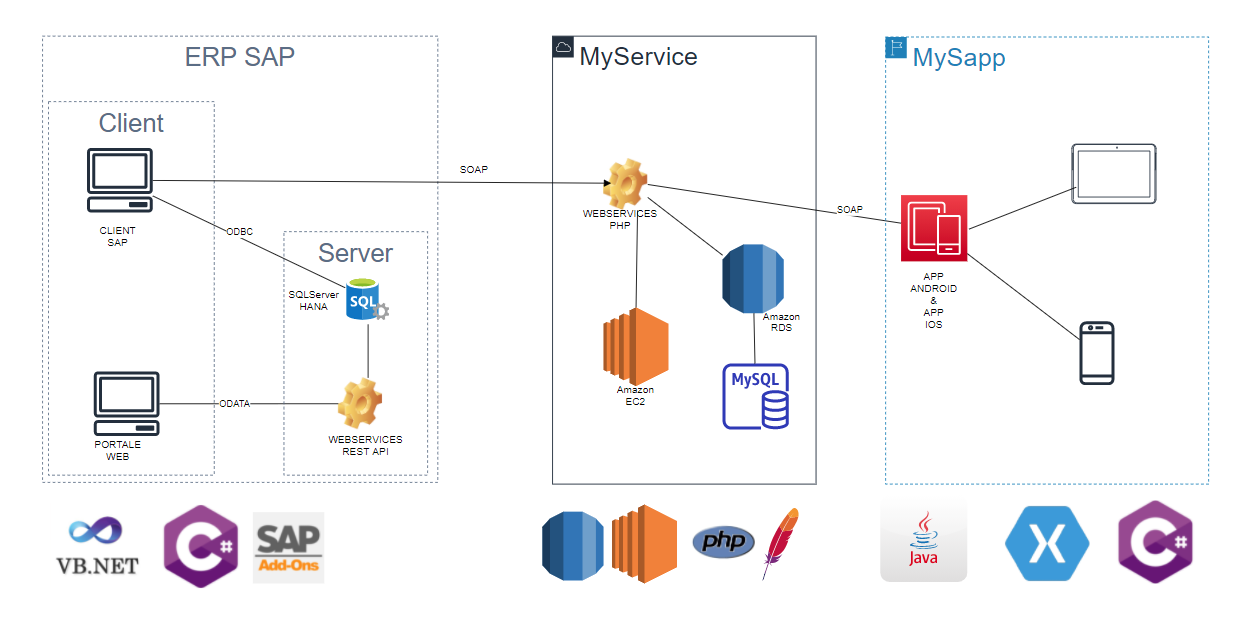
\includegraphics[scale = 0.4]{immagini/architettura-globale.png} 
	\caption{Schema di rappresentazione modulo gestionale ERP SAP, e moduli aggiunti dall'azienda intorno al gestionale}
\end{figure}\\
Da quest'immagine possiamo notare i tre moduli principali:
\begin{itemize}
	\item \textbf{ERP SAP:} il modulo del gestionale;
	\item \textbf{MyService:} il modulo dei webservices \gls{aws};
	\item \textbf{MySapp:} il modulo delle applicazioni Android e iOS.\\
\end{itemize}
Sulle due parti evidenziate dal cerchio rosso si è basato il mio lavoro in questo stage.
Nel client SAP verrà applicato l'applicazione add-on, mentre nei webservices php sono state effettuate delle modifiche ad alcune funzioni.
\section{Descrizione modulo ERP SAP}
\begin{figure}[!h] 
	\centering 
	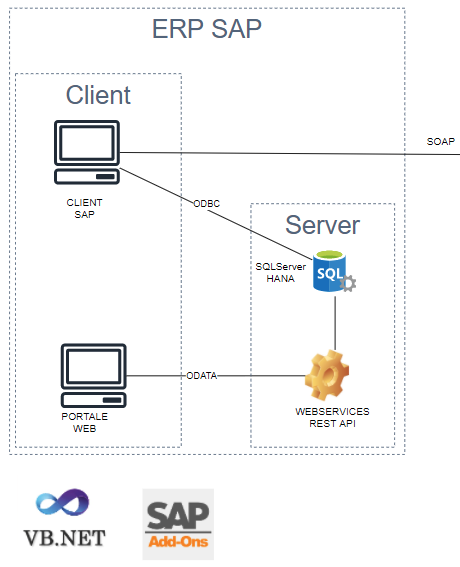
\includegraphics[scale = 1.2]{immagini/modulo-sap.png} 
	\caption{Schema di rappresentazione modulo gestionale ERP SAP}
\end{figure}

\subsection{ERP SAP}
\vspace{1em}
ERP SAP rappresenta il modulo del gestionale, in particolare nel nostro caso abbiamo come gestionale il SAP Business One.\\
ERP è l'acronimo di Enterprise Resource Planning.\\SAP è l'acronimo di Systems, Applications, Products.\\\\
SAP è un'azienda leader nel settore di ERP, e i suoi prodotti sono dei gestionali, ovvero dei software ERP.\\\\
Un software ERP è un tipo di software che le organizzazioni utilizzano per gestire le attività commerciali quotidiane, come ad esempio contabilità, project management, gestione del rischio e operazioni e gestione della catena di distribuzione.\\\\
Come possiamo vedere in Figura 2.2, il SAP è suddiviso in client e server.\\
Il server può essere basato su :
\begin{itemize}
	\item \textbf{SQLServer:} solo su Windows;
	\item \textbf{HANA:} solo su Linux.
\end{itemize}
Il client SAP attualmente è disponibile solo su Windows.\\Sul client SAP possono essere applicati degli add-on, per modificare i comportamenti della GUI del client in base a com'è programmato l'add-on.\\\\
I due gestionali più famosi di SAP sono:
\begin{itemize}
	\item SAP R/3;
	\item SAP Business One.
\end{itemize}
Questo progetto di stage è stato incentrato intorno al SAP Business One, dunque ora entreremo più nel dettaglio, su quest'ultimo.
\newpage
\subsection{SAP Business One}
SAP Business One, abbreviato a SAB B1, è un sofware ERP basato sulle piccole/medie imprese.
\\\\Questo gestionale è attualmente alla versione 10, rilasciata a marzo 2020, e rispetto al SAP R/3 consente molte più personalizzazione per essere adatto alle esigenze più disparate.
\\\\Come detto in precedenza è un tipico software con modello Client-server.
\begin{itemize}
	\item Il client è principalmente il Client SAP, o B1 Client, ma può essere anche un portale web oppure un'applicazione mobile;
	\item Il server viene eseguito su un database Microsoft SQL Server (Windows) oppure un database SAP HANA (Linux).\\
\end{itemize}
Infine, come detto in precedenza, SAB B1 consente di effettuare molte personalizzazioni (ovvero gli add-on) utilizzando \textbf{SAP Business One SDK}, ovvero un insieme di strumenti e librerie disponibili per lo sviluppo di add-ons su Microsoft Visual Studio, con C\# o VB.NET.\\\\
\begin{figure}[!h] 
	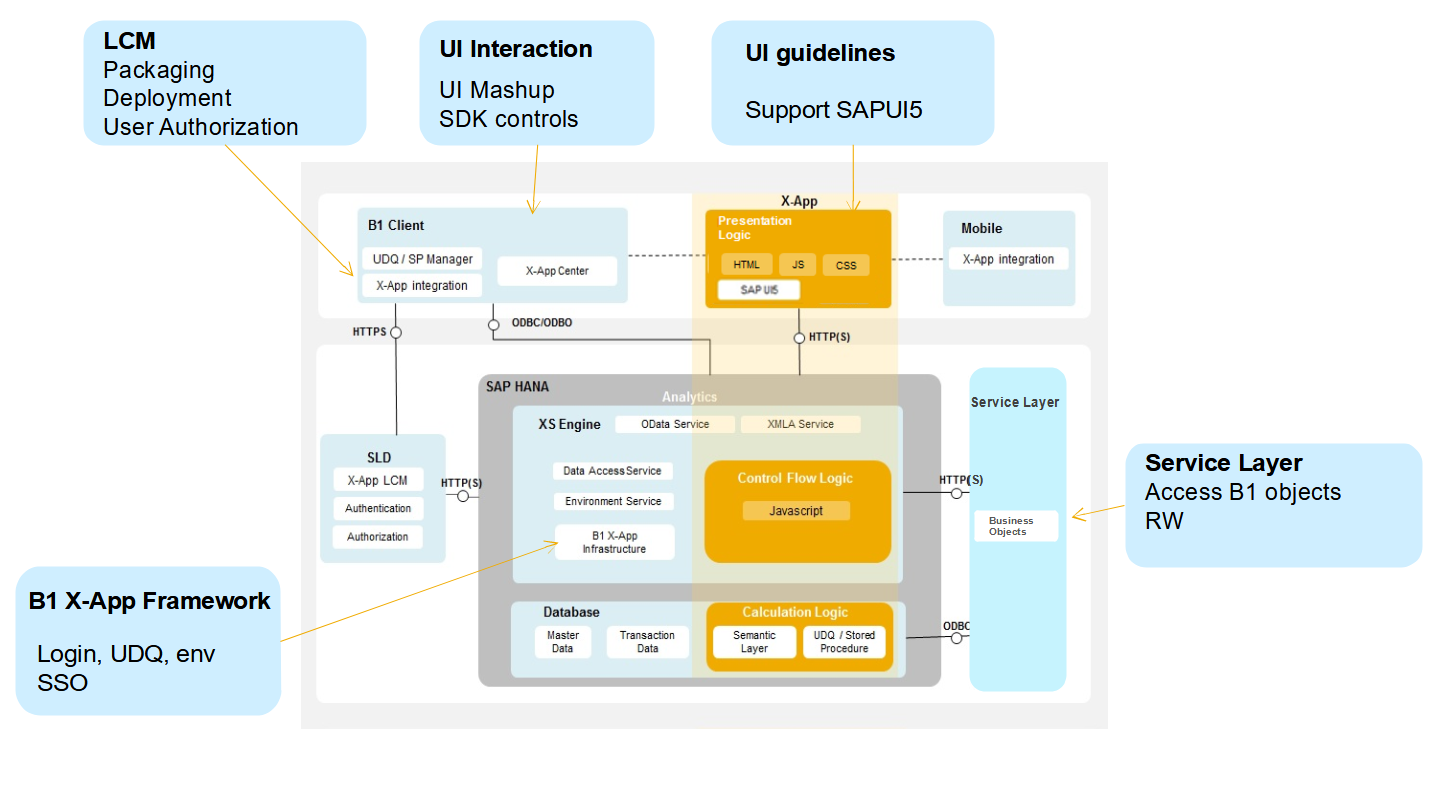
\includegraphics[scale = 0.4, left]{immagini/erp-sap-inside.png} 
	\caption{Schema ufficiale sul SAP Business One}
\end{figure}
\newpage
\begin{flushleft}
	Qui possiamo vedere uno schema sul SAP Business One, ufficiale dalla documentazione SAP.\\
	Possiamo vedere i vari client con cui accedere al SAP:
\end{flushleft}

\begin{itemize}
	\item \textbf{B1 Client:} ovvero il client SAP desktop;
	\item \textbf{X-APP:} ovvero un portale web sviluppato da SAP;
	\item \textbf{X-APP per mobile:} l'integrazione X-APP, per i dispositivi mobile;
	\item \textbf{Service Layer:} i webservices REST API, che possono essere utilizzati a loro volta da altre applicazioni (ad esempio, sito web o applicazioni mobile), per accedere al SAP.
\end{itemize}
Tutti questi client accedono al SAP attraverso vie diverse.
\begin{itemize}
		\item Il client SAP, B1 Client, accede al database attraverso:
		\begin{enumerate}
			\item \gls{odbc} 
			\item \gls{odbo}
		\end{enumerate}
		e successivamente accede a SLD, ovvero la componente di autenticazione, via HTTP(S);
\item I webservices accedono al server SAP attraverso HTTP(S), e ricevono risposta dal database attraverso \gls{odbc};
	\item X-APP, sia versione web che mobile, accede al server SAP, e quindi successivamente al database, attraverso HTTP(S).
\end{itemize}
In questa figura, si può XS Engine, ovvero il server SAP (la logica SAP) e il database, contenuti dentro il DBMS SAP HANA, ma lo stesso vale se il DBMS è Microsoft SQL Server.\\
Ora proseguiamo analizzando le componenti principali del SAP, ovvero:
\begin{itemize}
	\item il client SAP;
	\item il server SAP;
	\item il Service Layer di SAP, ovvero i webservices REST API.
\end{itemize}
\newpage
\subsection{Client SAP}
\begin{flushleft}
	\item Il client SAP utilizza la connessione \gls{odbc} per comunicare con il server SAP.\\ODCB, ovvero Open DataBase Connectivity, è uno standard utilizzato per la connessione tra client e DBMS. 
	\item Mentre utilizza il protocollo \gls{soap} per comunicare con il webserver \gls{aws} del modulo MyService.
\end{flushleft}
\begin{figure}[!h] 
	\centering 
	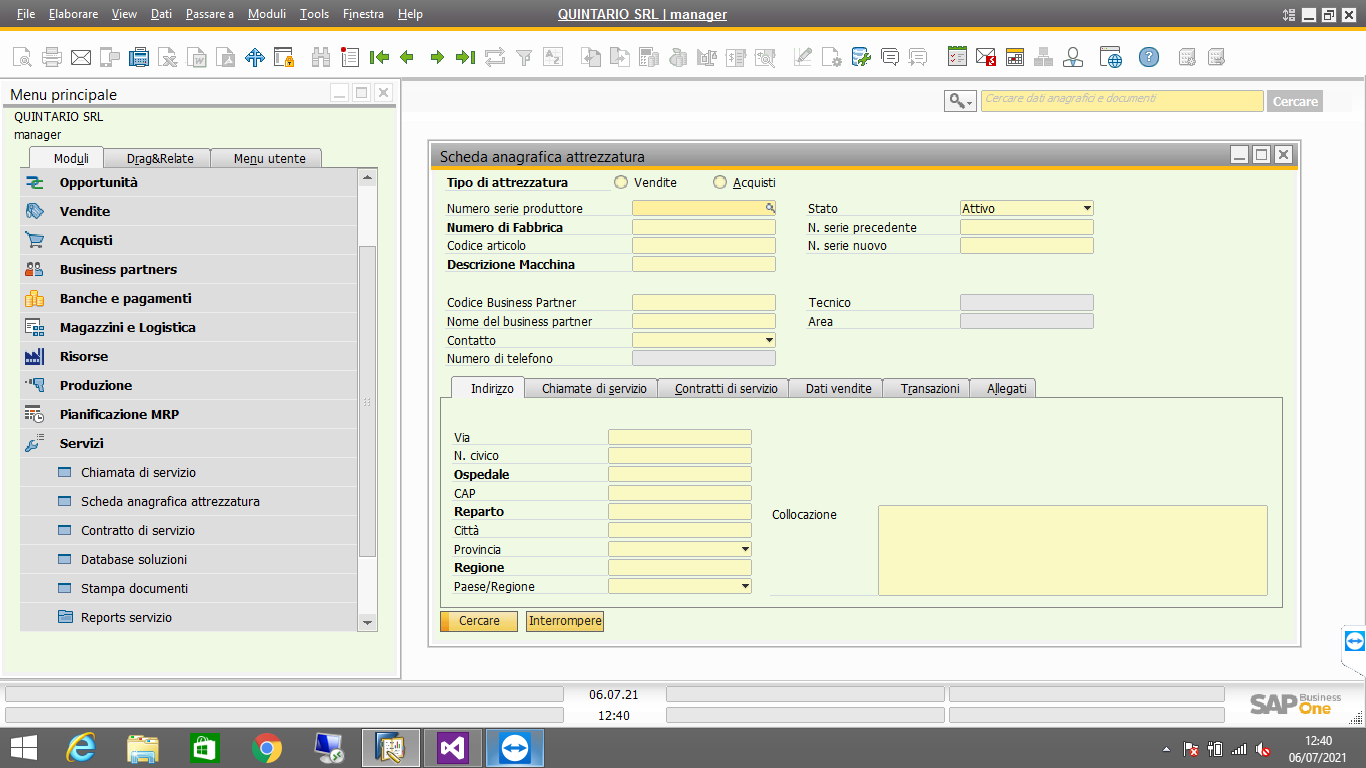
\includegraphics[scale = 0.4]{immagini/client-sap.png} 
	\caption {Client SAP, aperto sulla scheda "Scheda anagrafica attrezzatura"}
\end{figure}
\begin{flushleft}
	\item Qui possiamo vedere come appare il Client SAP.\\In questo caso è stata aperta la Scheda anagrafica attrezzatura, del modulo dei Servizi.\\Da notare che questi "moduli" del SAP, differiscono dai moduli coinvolti con il modulo del gestionale (MyService e MySapp), questi sono moduli interni del SAP.
	\item La scheda anagrafica attrezzatura è una scheda che rappresenta le attrezzature dell'azienda, ad esempio macchine a controllo numerico, lavatrici o condizionatori, e tutti i possibili macchinari dell'azienda.
	\item Ora vediamo un esempio di cambiamento della GUI di questo client con l'applicazione di un Add-On alla scheda anagrafica attrezzatura.
\end{flushleft}
\pagebreak
\begin{figure}[!h] 
	\centering 
	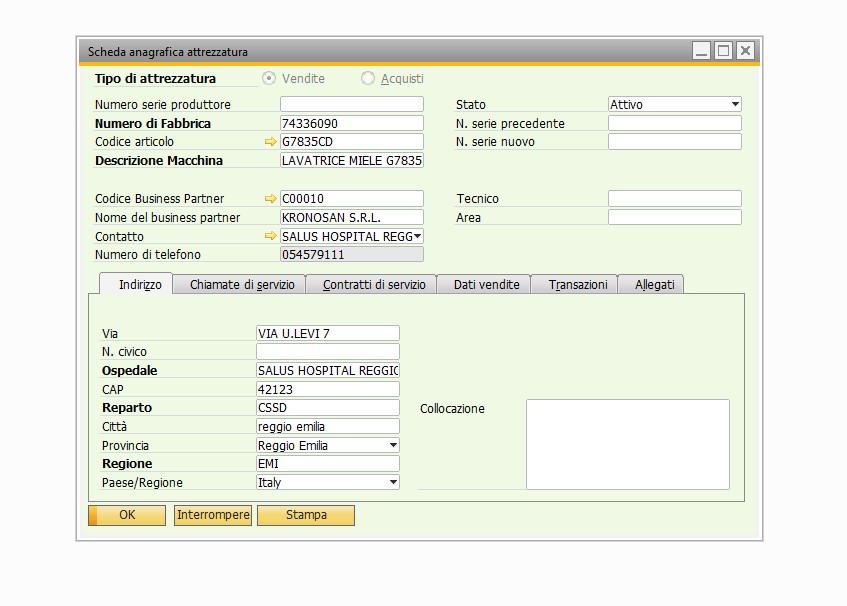
\includegraphics[scale = 0.6]{immagini/esempio-modifica-client-addon.jpg} 
	\caption {Client SAP, esempio di modifica GUI di un add-on applicato sulla scheda "Scheda anagrafica attrezzatura"}
\end{figure}
\begin{flushleft}
	\item Come possiamo vedere è apparso un nuovo pulsante, che stamperà i dati della scheda.\\Questo è un'esempio molto semplice, ma si possono cambiare altre cose, ad esempio aggiungere o rimuovere campi, o aggiungere funzioni ad eventi, ad esempio messaggi di testo che appaiono cliccando dei campi particolari.
	\item Questi add-on possono essere programmati tramite Microsoft Visual Studio, con :
	\begin{itemize}
		\item \textbf{C\#}, C sharp;
		\item \textbf{VB.NET}, Visual Basic NET.
	\end{itemize}
\end{flushleft}
\newpage
\subsection{Portale Web}
Ora mostriamo il portale web, sviluppato dall'azienda, in concomitanza con un'altra azienda specializzata in siti web (mys).\\
L'admin del portale, oppure l'admin relativo all'azienda cliente, crea le credenziali per i vari utenti, che saranno i dipendenti delle aziende clienti di Sinapsi.\\
Dunque arrivati al sito web, bisogna inserire le credenziali nella sezione Login, che apparirà come prima pagina del sito.\\
\begin{figure}[!h] 
	\centering 
	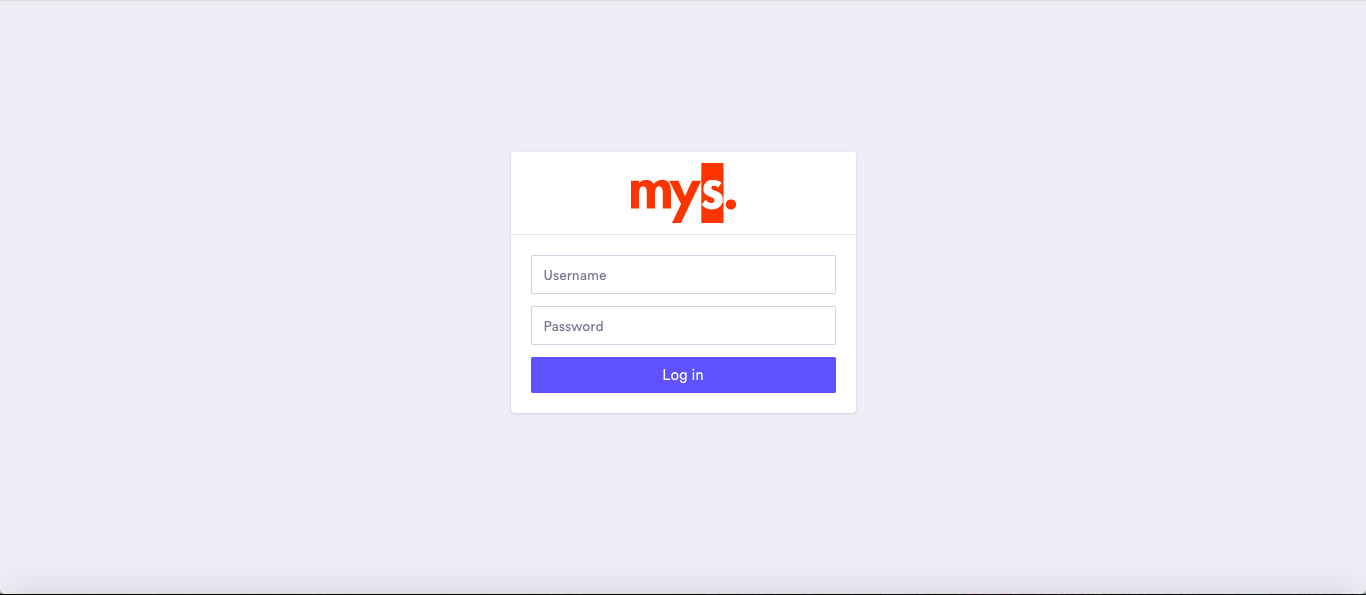
\includegraphics[scale = 0.3]{immagini/portale/login.png} 
	\caption {Portale Web, sezione di Login}
\end{figure}
\\Una volta effettuato il login, si viene reindirizzati al sito web, vero e proprio.\\
Da qui abbiamo principalmente 3 schermate principali:
\begin{itemize}
	\item Attrezzature;
	\item Calendario;
	\item Interventi.\\
\end{itemize}
La schermata Attrezzature mostra in forma tabellare, tutte le attrezzature e macchinari dell'azienda, con i vari dettagli.\\\\
La schermata Interventi mostra sempre in forma tabellare, i vari interventi richiesti su quale attrezzatura, e i dettagli dell'intervento.\\
E' presente un altra sezione, nella schermata Interventi, la sezione Interventi In Attesa, che mostra gli interventi che si stanno sincronizzando con il database SAP, che non sono ancora sincronizzati.
\newpage
Cominciamo con la schermata Calendario, qui sotto.\\
\begin{figure}[!h] 
	\centering 
	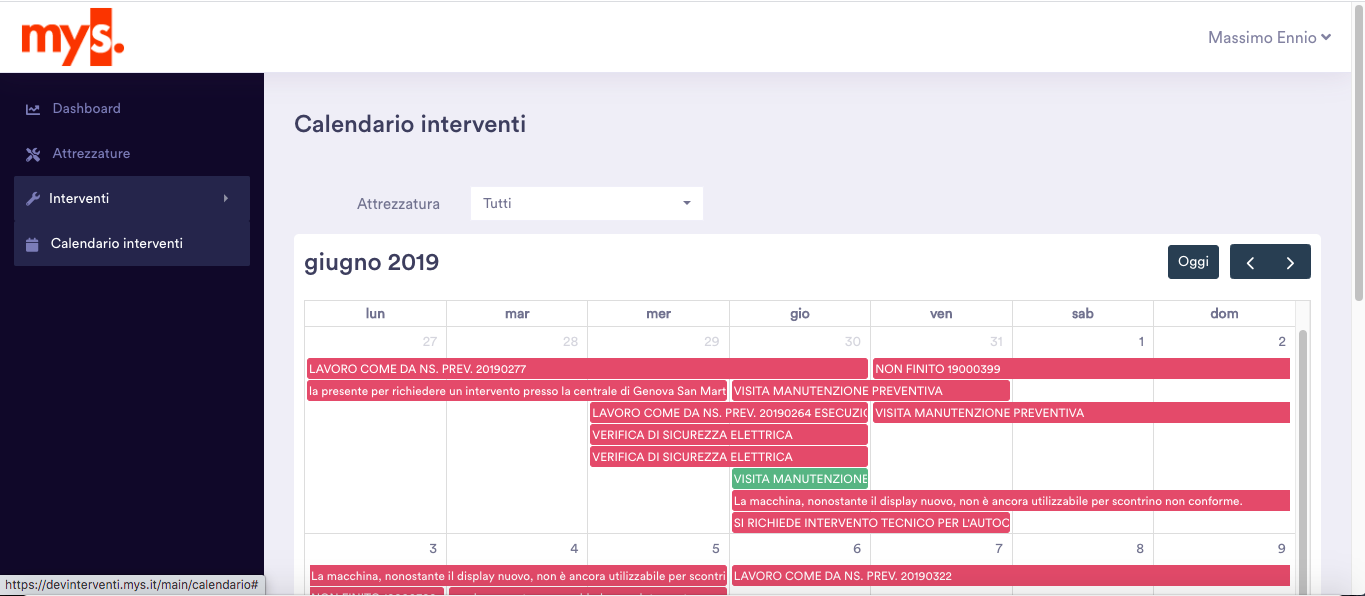
\includegraphics[scale = 0.3]{immagini/portale/calendario.png} 
	\caption {Portale Web, schermata Calendario}
\end{figure}
\\Evidenziate di rosso ci sono le chiamate di servizio, ad esempio manutenzioni, non completate, mentre evidenziate in verde quelle completate.\\\\
Ora continuiamo con la schermata Attrezzature.\\
\begin{figure}[!h] 
	\centering 
	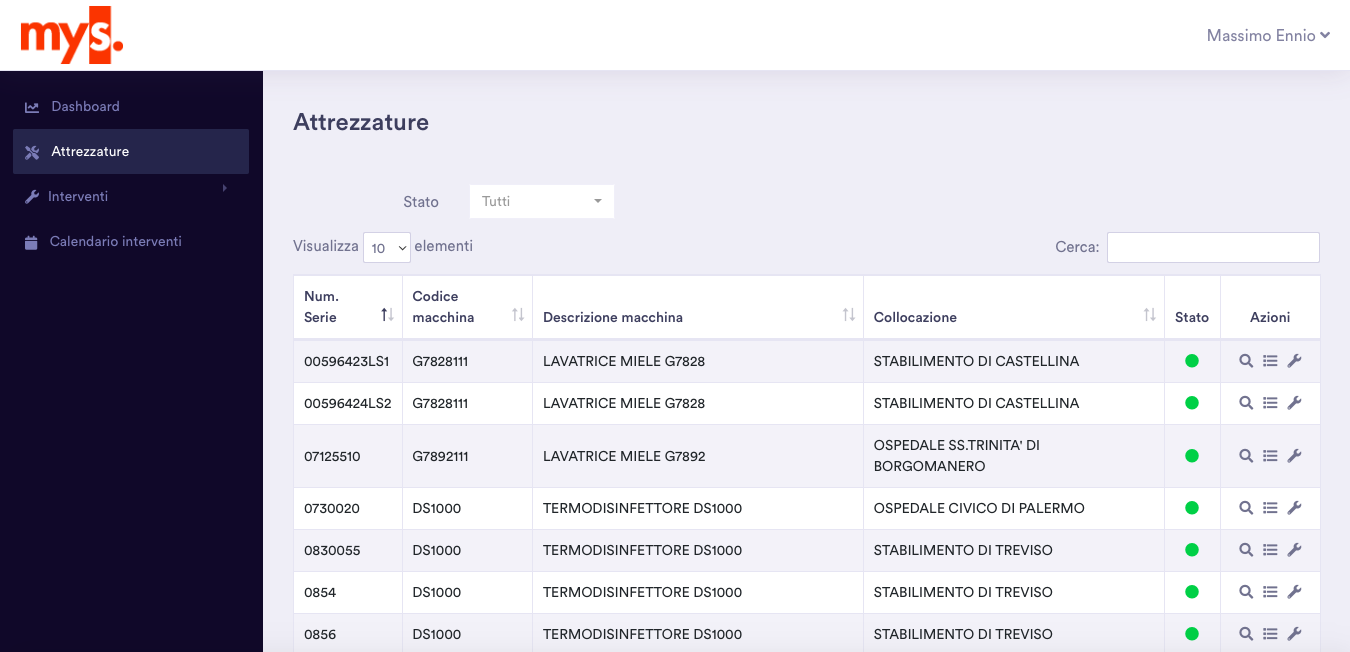
\includegraphics[scale = 0.25]{immagini/portale/attrezzature.png} 
	\caption {Portale Web, schermata Attrezzature}
\end{figure}
\\Qui possiamo vedere tutte le attrezzature, relative all'azienda cliente collegata, e quindi alle credenziali.\\
Per ogni attrezzatura ci sono alcune azioni, tra cui ricerca ed elenco chiamate di servizio.\\Tra le varie azioni la più interessante è l'apertura di una nuova chiamata di servizio, ovvero richiedere un nuovo intervento, ad esempio una manutenzione o sostituzione di componenti.\\\\
Ora passiamo alla schermata degli interventi, di cui possiamo conoscerne tutte le caratteristiche principali, come numero e tipo di intervento, data inizio e fine.\\
E anche la causale e lo stato, per stato si intende se l'intervento è già stato effettuato.
\begin{figure}[!h] 
	\centering 
	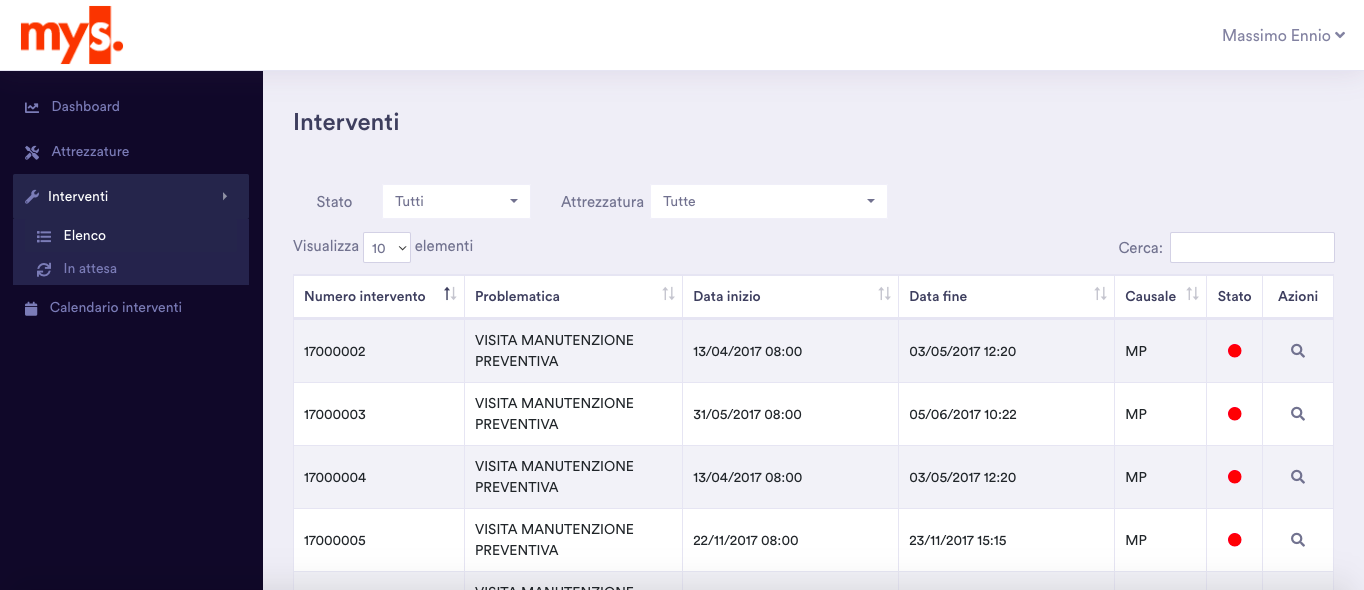
\includegraphics[scale = 0.25]{immagini/portale/interventi.png} 
	\caption {Portale Web, sezione di Login}
\end{figure}
\\\\Infine, all'interno della schermata degli interventi, abbiamo la sezione "In attesa", per gli interventi in attesa di sincronizzazione.\\
Questi sono gli interventi creati tramite questo portale web, che si stanno sincronizzando con il server SAP, lo stato verde indicano che si sono sincronizzati, quello rosso che non si sono ancora sincronizzati.
\begin{figure}[!h] 
	\centering 
	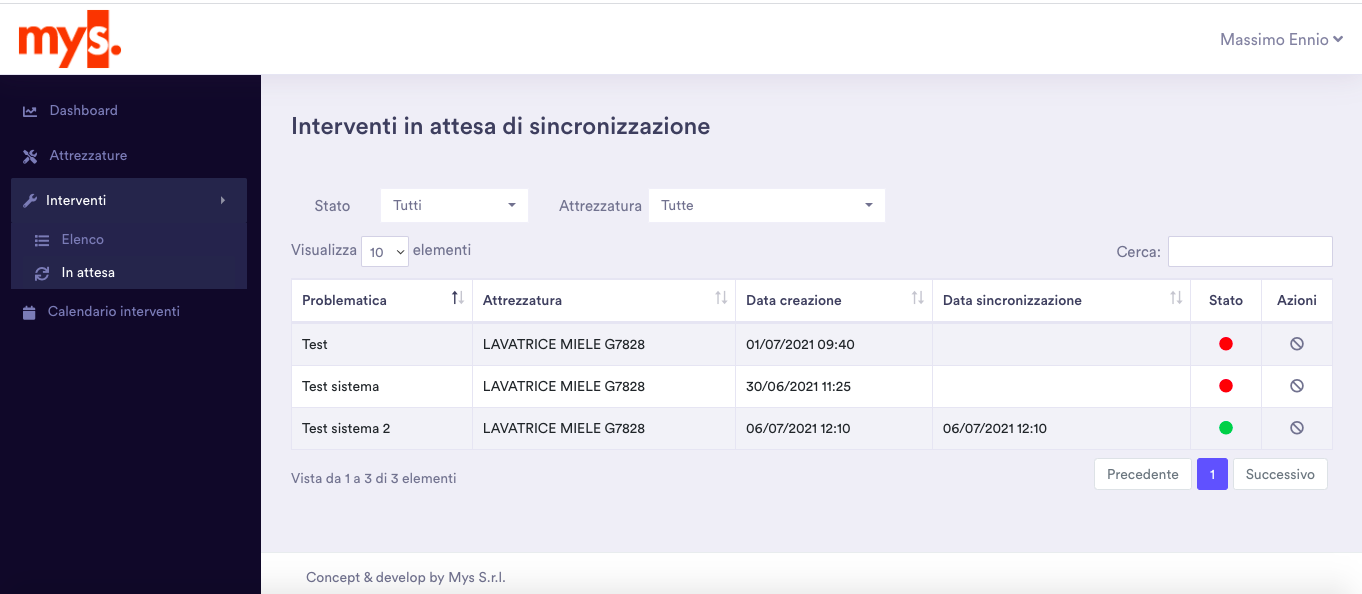
\includegraphics[scale = 0.25]{immagini/portale/interventi-in-attesa.png} 
	\caption {Portale Web, schermata Interventi, sezione In attesa}
\end{figure}
\pagebreak
\subsection{Webservices REST API}
\begin{flushleft}
	\item Recentemente, su SAP Business One è stato introdotto un service layer, composto da webservices REST API, che comunicano tramite protocollo ODATA (open data protocol).
	\item Questi webservices permettono di accedere direttamente agli oggetti SAP,\\senza passare per il client SAP.\\Gli oggetti SAP sono una struttura dati generata dalla logica del server SAP, \\che raggruppano e ordinano secondo certe logiche i dati presenti nel database.
	\\ Per poter ottenere questi dati bisogna fare una richiesta http al webserver, il quale invierà un file json con gli oggetti SAP richiesti.
	\\L'utilizzo più comune di questi webservices è un portale web che usi le informazioni prese tramite queste richieste HTTP. 
\end{flushleft}
\begin{figure}[!h] 
	\centering 
	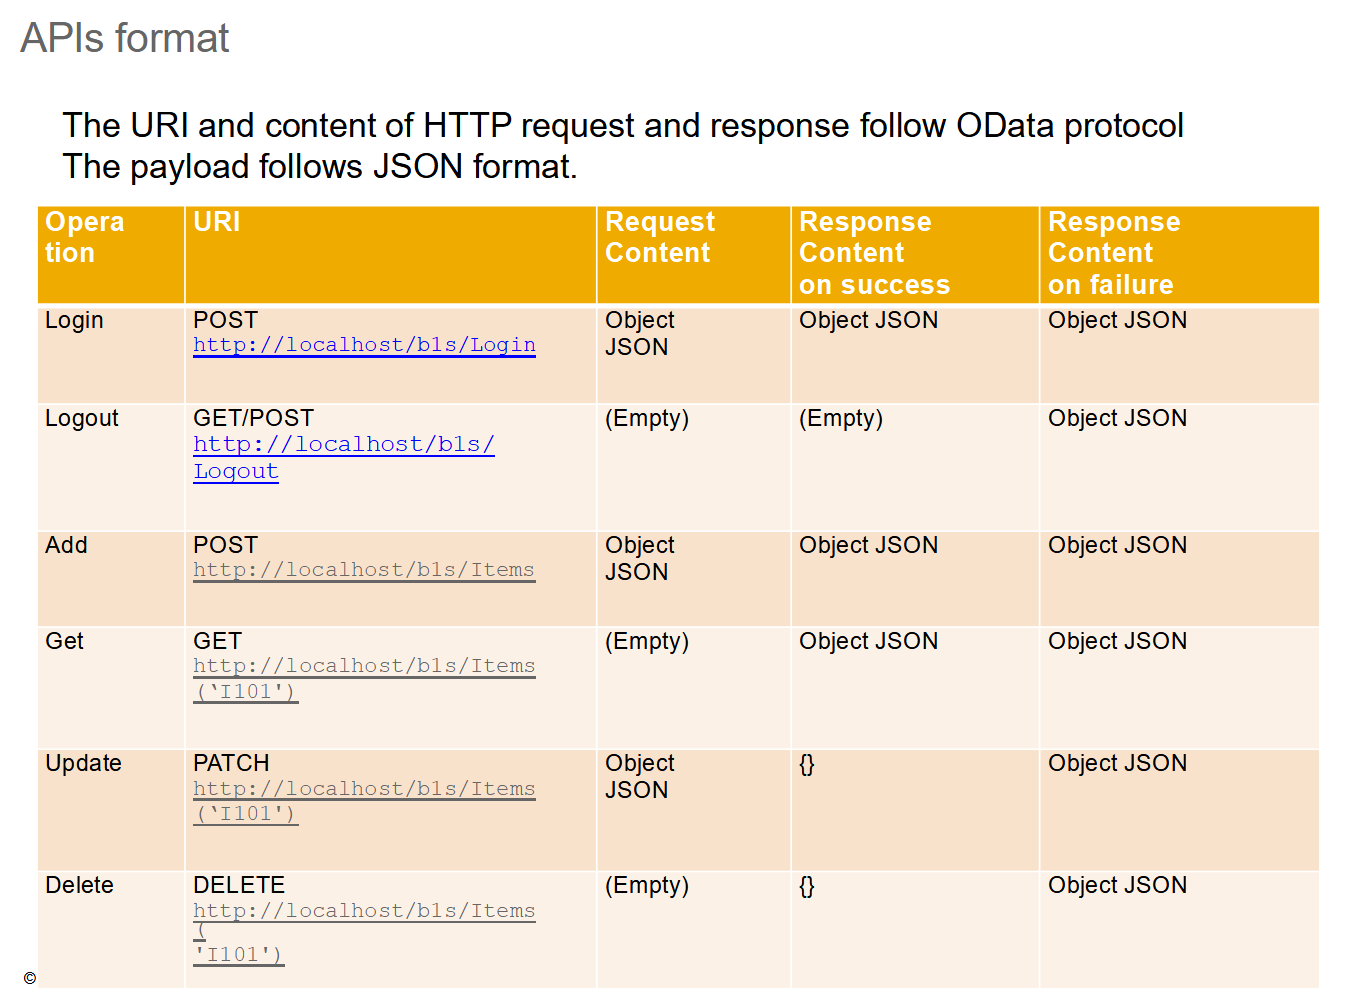
\includegraphics[scale = 0.37]{immagini/api_Format.png} 
	\caption {Formato delle richieste HTTP per il Service Layer SAP}
\end{figure}
\begin{flushleft}
	\item Come si può osservare da quest'immagine, sono presenti le richieste HTTP principali per interagire con i webservices REST API del Service Layer di SAP.
	\item A seguito di una richiesta HTTP viene elaborata la richiesta.\\Viene restituito un oggetto JSON in caso di fallimento, comunicando l'errore causante il fallimento.\\In caso di successo viene restituito un oggetto JSON, ove necessario, oppure un messaggio vuote che rappresenta il successo dell'operazione.
\end{flushleft}
\section{Descrizione modulo MyService}
\begin{figure}[!h] 
	\centering 
	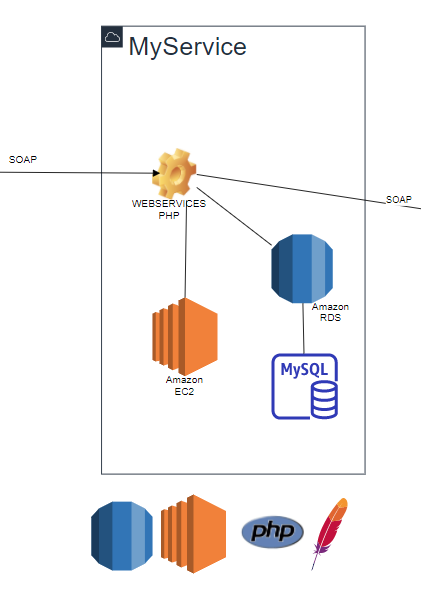
\includegraphics[scale = 1.1]{immagini/modulo-myservice.png} 
	\caption{Schema di rappresentazione modulo MyService dei servizi \gls{aws}}
\end{figure}
\newpage
\subsection{Servizi AWS}
In questo modulo abbiamo i webservices in PHP installati in un server \gls{aws}, accompagnato da un database MySQL.
\gls{aws} è un acronimo che sta per Amazon Web Services.
In particolare, dei servizi \gls{aws}, in questo modulo abbiamo:
\begin{itemize}
	\item Amazon \gls{ec2}, Amazon Elastic Compute Cloud, che consiste nel webserver, ovvero il server dove sono presenti i nostri webservices in php;
	\item Amazon \gls{rds}, Amazon Relational Database Service, che si occupa della gestione del database MySQL;
	\item Amazon \gls{s3}, Amazon Simple Storage Service, che nello schema non è presente, ma si occupa della gestione di allegati e file troppo pesanti nel database per essere gestiti da Amazon \gls{rds}.
\end{itemize}
Ora rivolgiamo la nostra attenzione ai webservices PHP, che mettono in relazione questo webserver e il database con il modulo SAP e il modulo MySapp, delle applicazioni mobile, attraverso il protocollo \gls{soap}.
\subsection{Webservices PHP}
Come possiamo vedere dalla figura del modulo MyService e dalla figura generale dell'infrastruttura preeesistente, il client SAP comunica con questi webservices PHP, attraverso un add-on che utilizza il protocollo \gls{soap}.\\
Per programmare questi webservices sono state utilizzate le tecnologie Apache e PHP.\\ 
Il protocollo \gls{soap}, ovvero Simple Object Access Protocol, è un protocollo per lo scambio di messaggi tra componenti software.\\\\
I webservices php comunicano anche con le applicazioni mobile, per Android e iOS, sempre tramite protocollo \gls{soap}.\\
Vi sono moltissime funzioni in PHP che corrispondono a molte funzioni \gls{soap} nei webservices, il cui compito principale è mettere in relazione le app mobile o il SAP, con il database contenuto in questo modulo.\\
L'obiettivo principale è gestire le chiamate di servizio, ovvero richieste di intervento, ai tecnici del SAP.\\
Elenchiamo alcune delle funzioni più comuni:
\begin{itemize}
	\item Visione di tutti i dettagli di una chiamata di servizio;
	\item Visione di tutte le chiamate di servizio di un tecnico;
	\item Rimozione di una chiamata di servizio;
	\item Modifica di una chiamata di servizio;
	\item Aggiunta di una chiamata di servizio;
	\item Invio mail a cliente, una volta concluso una chiamata di servizio;
	\item Login di un tecnico;
	\item Logout di un tecnico.
\end{itemize}
\newpage
\section{Descrizione modulo MySapp}
\begin{figure}[!h] 
	\centering 
	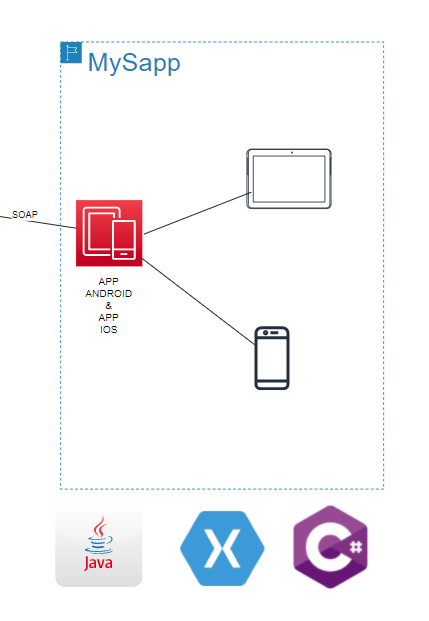
\includegraphics[scale = 1.1]{immagini/modulo-mysapp.png} 
	\caption{Schema di rappresentazione modulo MySapp delle applicazioni mobili}
\end{figure}
\newpage
\subsection{Applicazioni mobile}
Il modulo MyService si collega con questo modulo MySapp, attraverso il protocollo \gls{soap} utilizzando i webservices PHP del modulo MyService.\\
Sono state sviluppate due applicazioni per i clienti che risolvono le chiamate di servizio on-site, ovvero di persona.\\
In queste applicazioni, il tecnico esegue il login, con le sue credenziali e successivamente può gestire le chiamate di servizio a egli assegnate.\\
Ora vediamo velocemente com'è stato impostato il layout delle due applicazioni.
\subsubsection{Applicazione iOS}
Per lo sviluppo dell'applicazione iOS è stato utilizzando C\# e Xamarin.\\\\
Cominciamo con la schermata di login.\\
\begin{figure}[!h] 
	\centering 
	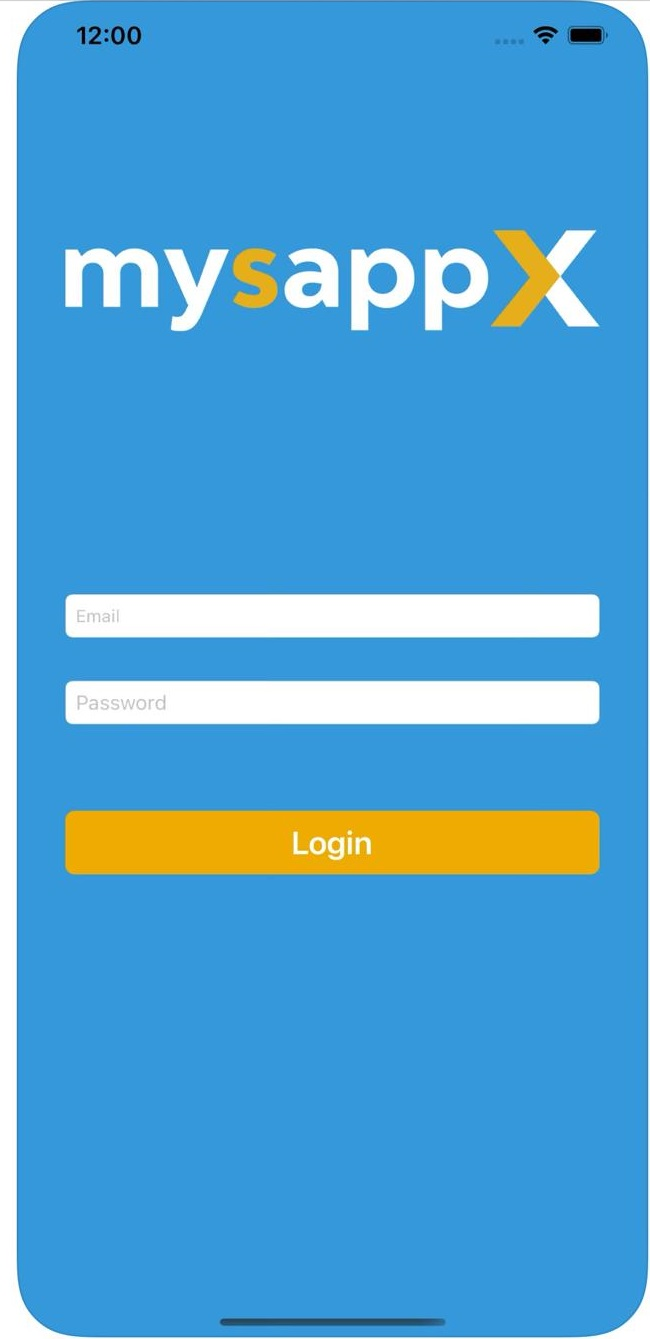
\includegraphics[scale = 0.2]{immagini/app iOS/login-iOS.jpeg} 
	\caption {App iOS, schermata di Login}
\end{figure}
\\Qui il tecnico dovrà inserire le proprie credenziali e accederà alla gestione delle chiamate di servizio a lui assegnate.
\newpage
\begin{flushleft}
	Continuiamo con la schermata Principale dell'app.
	\\In questa schermata si possono vedere le chiamate di servizio assegnate a questo tecnico ancora da eseguire.
\end{flushleft}
\begin{figure}[!h] 
	\centering 
	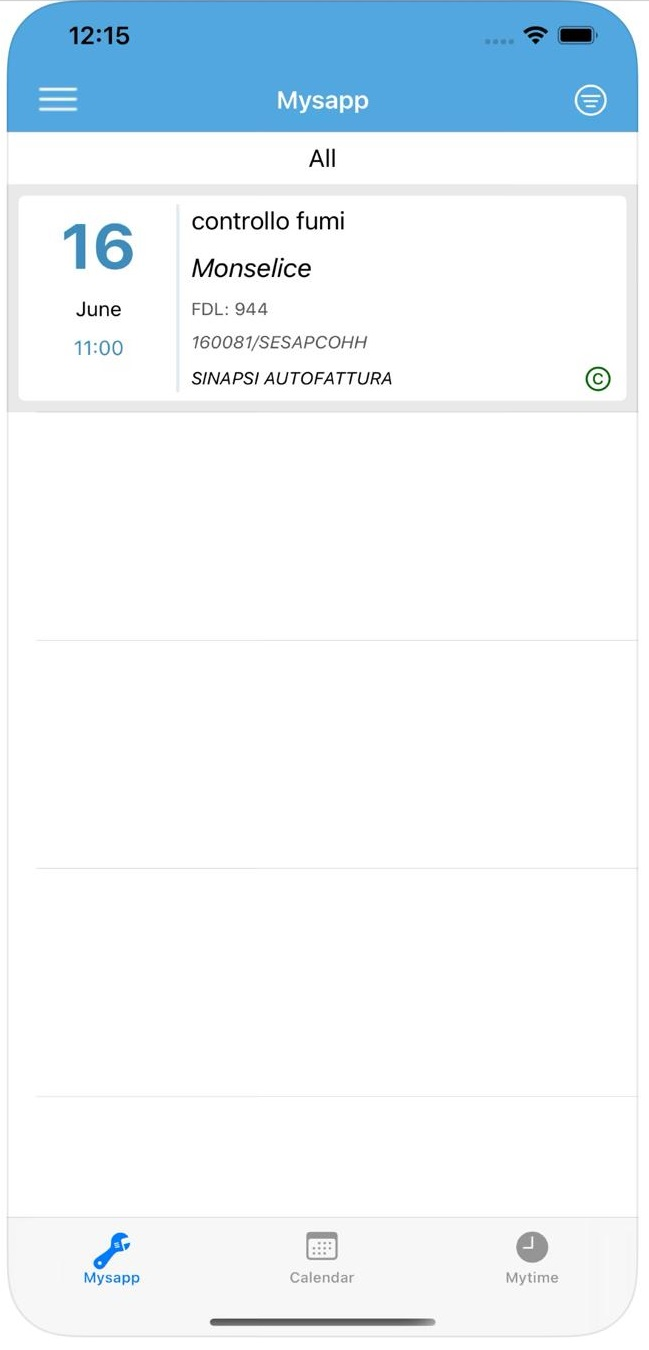
\includegraphics[scale = 0.13]{immagini/app iOS/elenco-interventi-iOS.jpeg} 
	\caption {App iOS, schermata Principale}
\end{figure}
Qui sotto possiamo vedere il calendario e la posizione della o delle chiamate di servizio da eseguire.\\
\begin{figure}[!h] 
	\centering 
	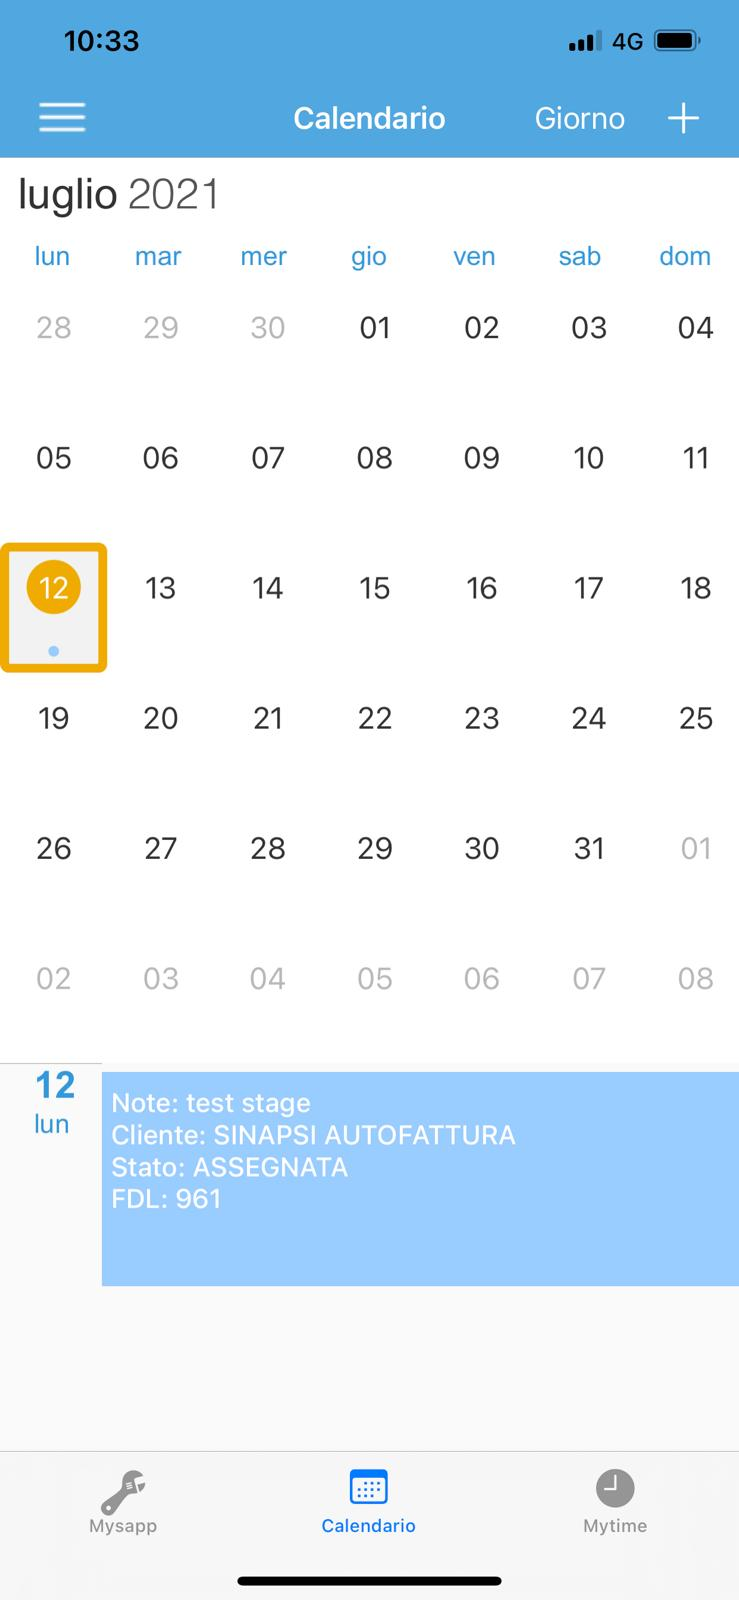
\includegraphics[scale = 0.13]{immagini/app iOS/calendario-iOS.jpeg} 
	\caption {App iOS, schermata Calendario}
\end{figure}
\newpage
Infine, abbiamo i dettagli della chiamata di servizio selezionata.\\
\begin{figure}[!h] 
	\centering 
	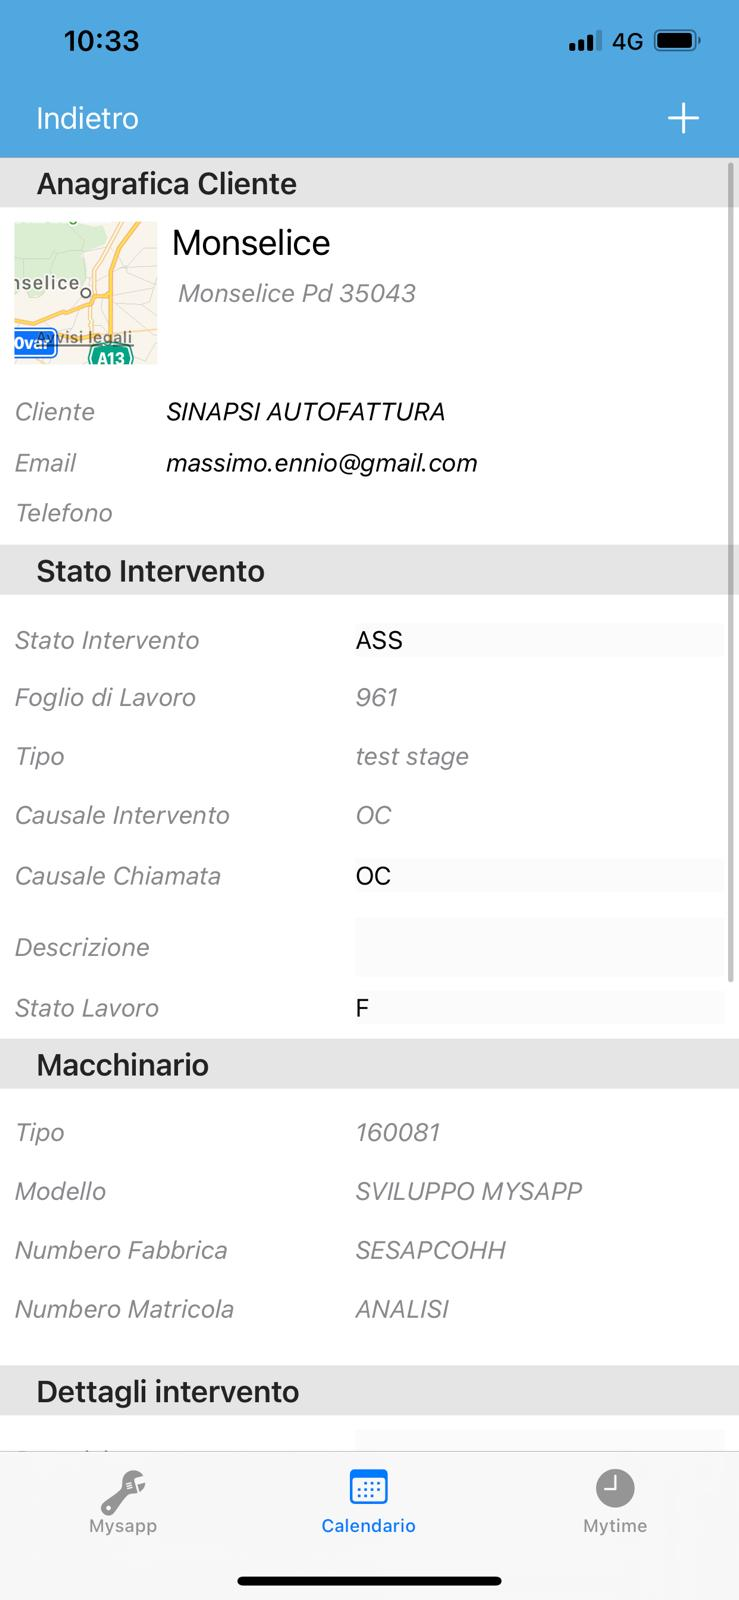
\includegraphics[scale = 0.2]{immagini/app iOS/intervento-iOS.jpeg} 
	\caption {App iOS, schermata Intervento}
\end{figure}
\\Qui possiamo vedere i vari dettagli della chiamata di servizio, ad esempio:
\begin{itemize}
	\item posizione del cliente;
	\item stato dell'intervento;
	\item attrezzatura che necessita dell'intervento;
	\item e altri dettagli meno importanti.
\end{itemize}
\newpage
\subsubsection{Applicazione Android}
Per lo sviluppo dell'applicazione Android è stato utilizzato Java e Kotlin.\\\\
Cominciamo a esplorare l'applicazione dalla schermata di login.\\
\begin{figure}[!h] 
	\centering 
	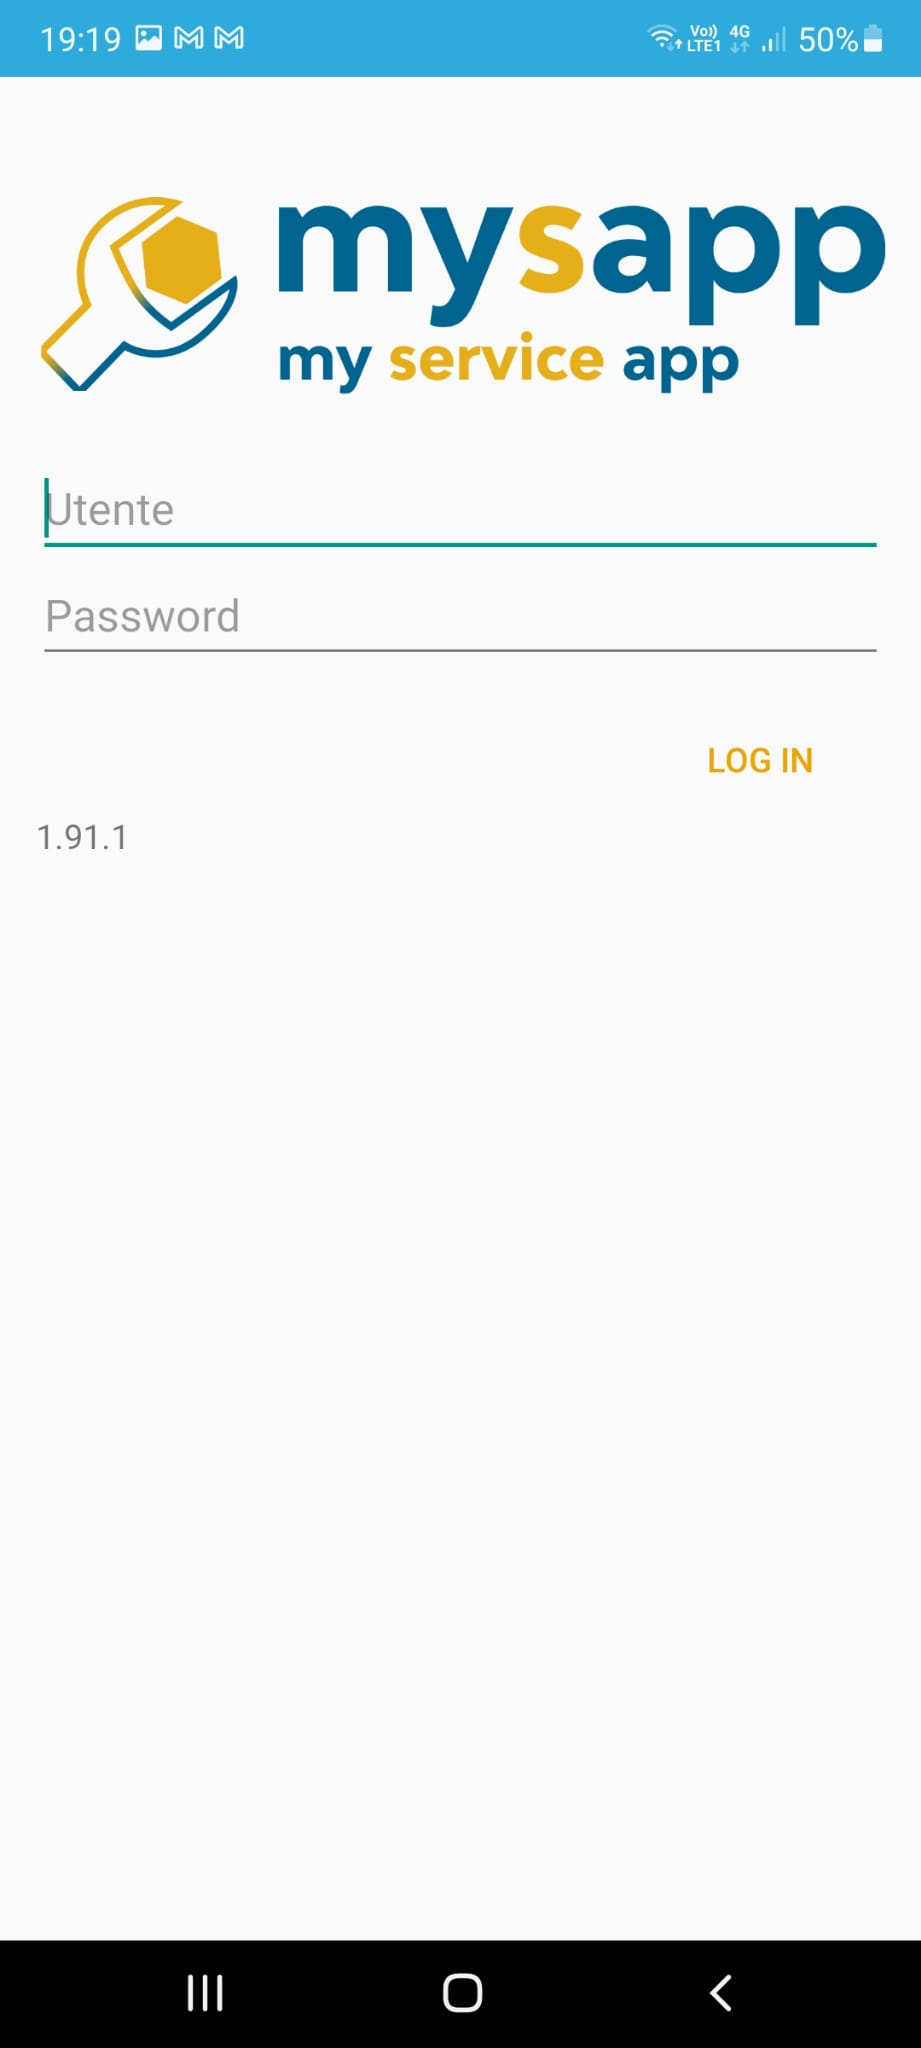
\includegraphics[scale = 0.2]{immagini/app Android/login-android.jpeg} 
	\caption {App Android, schermata di Login}
\end{figure}
Qui il tecnico dovrà inserire le proprie credenziali.\\
\newpage
\begin{flushleft}
	Continuiamo con la schermata Principale dell'app.\\
	La schermata dove si possono vedere le chiamate assegnate a questo tecnico.
\end{flushleft}
\begin{figure}[!h] 
	\centering 
	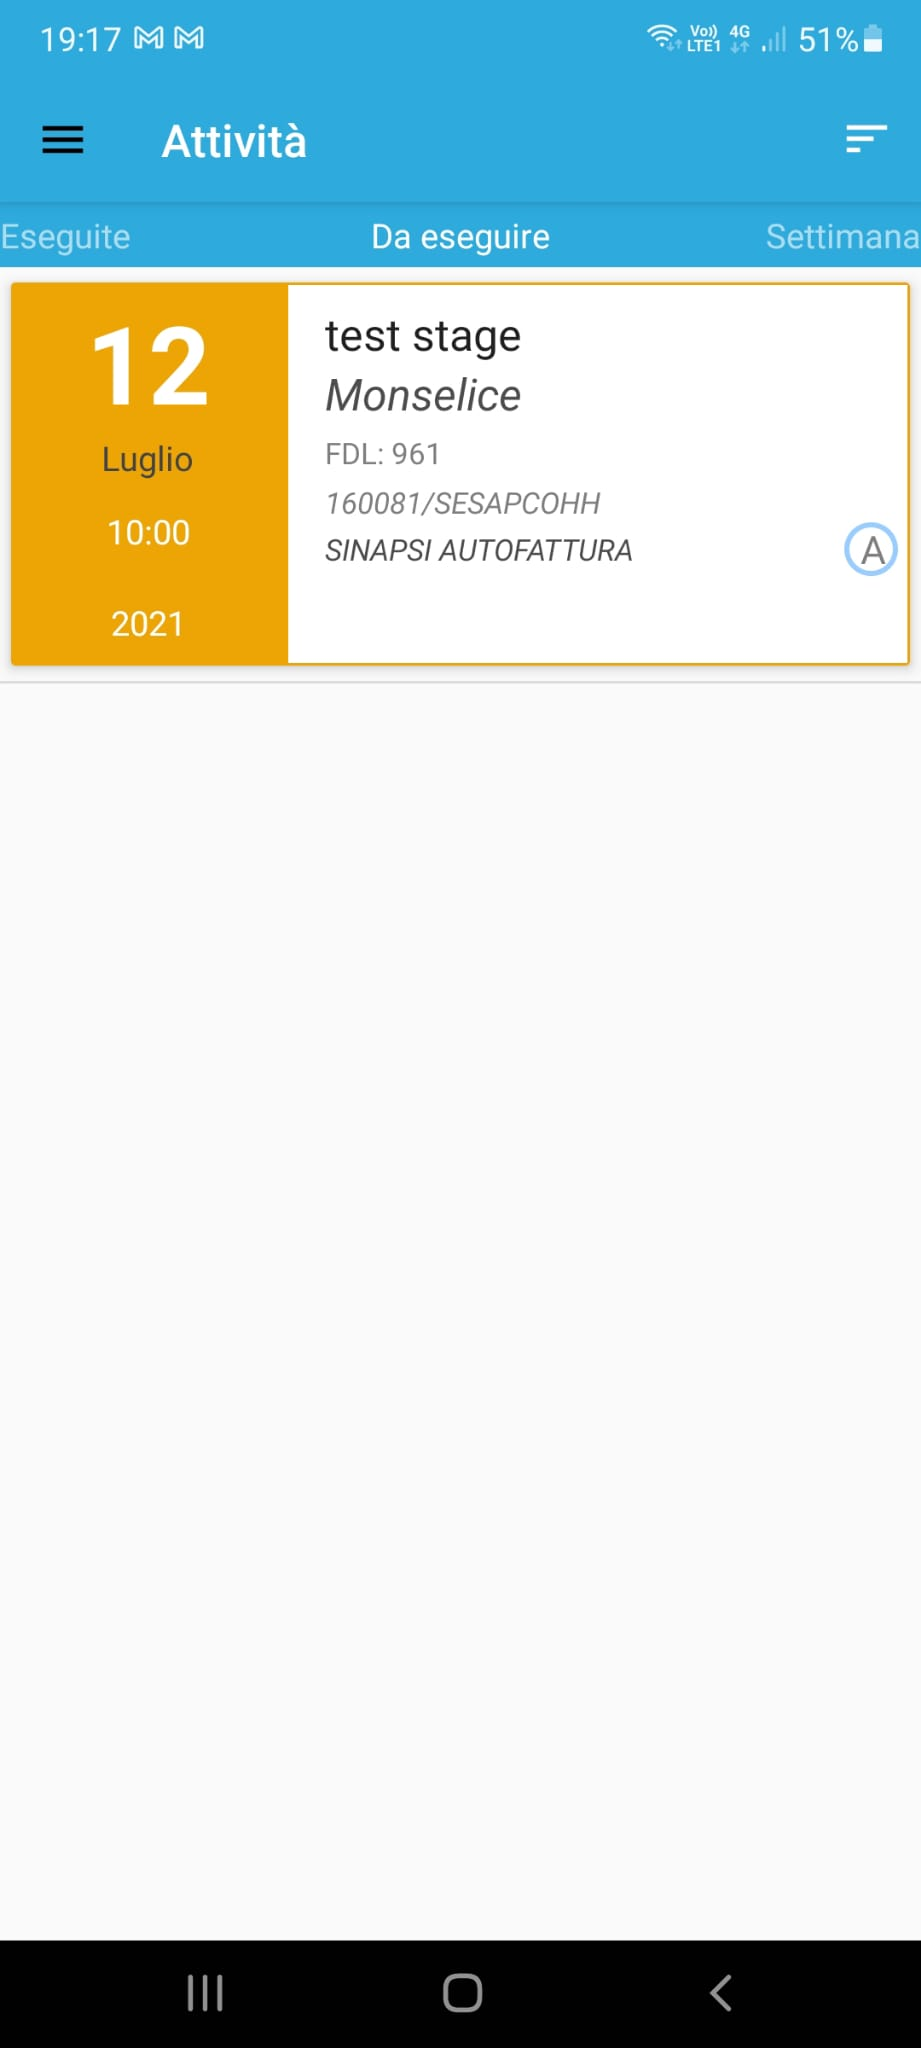
\includegraphics[scale = 0.11]{immagini/app Android/elenco-interventi-android.jpeg} 
	\caption {App Android, schermata Principale}
\end{figure}
Qui sotto possiamo vedere la schermata calendario dell'app.\\
\begin{figure}[!h] 
	\centering 
	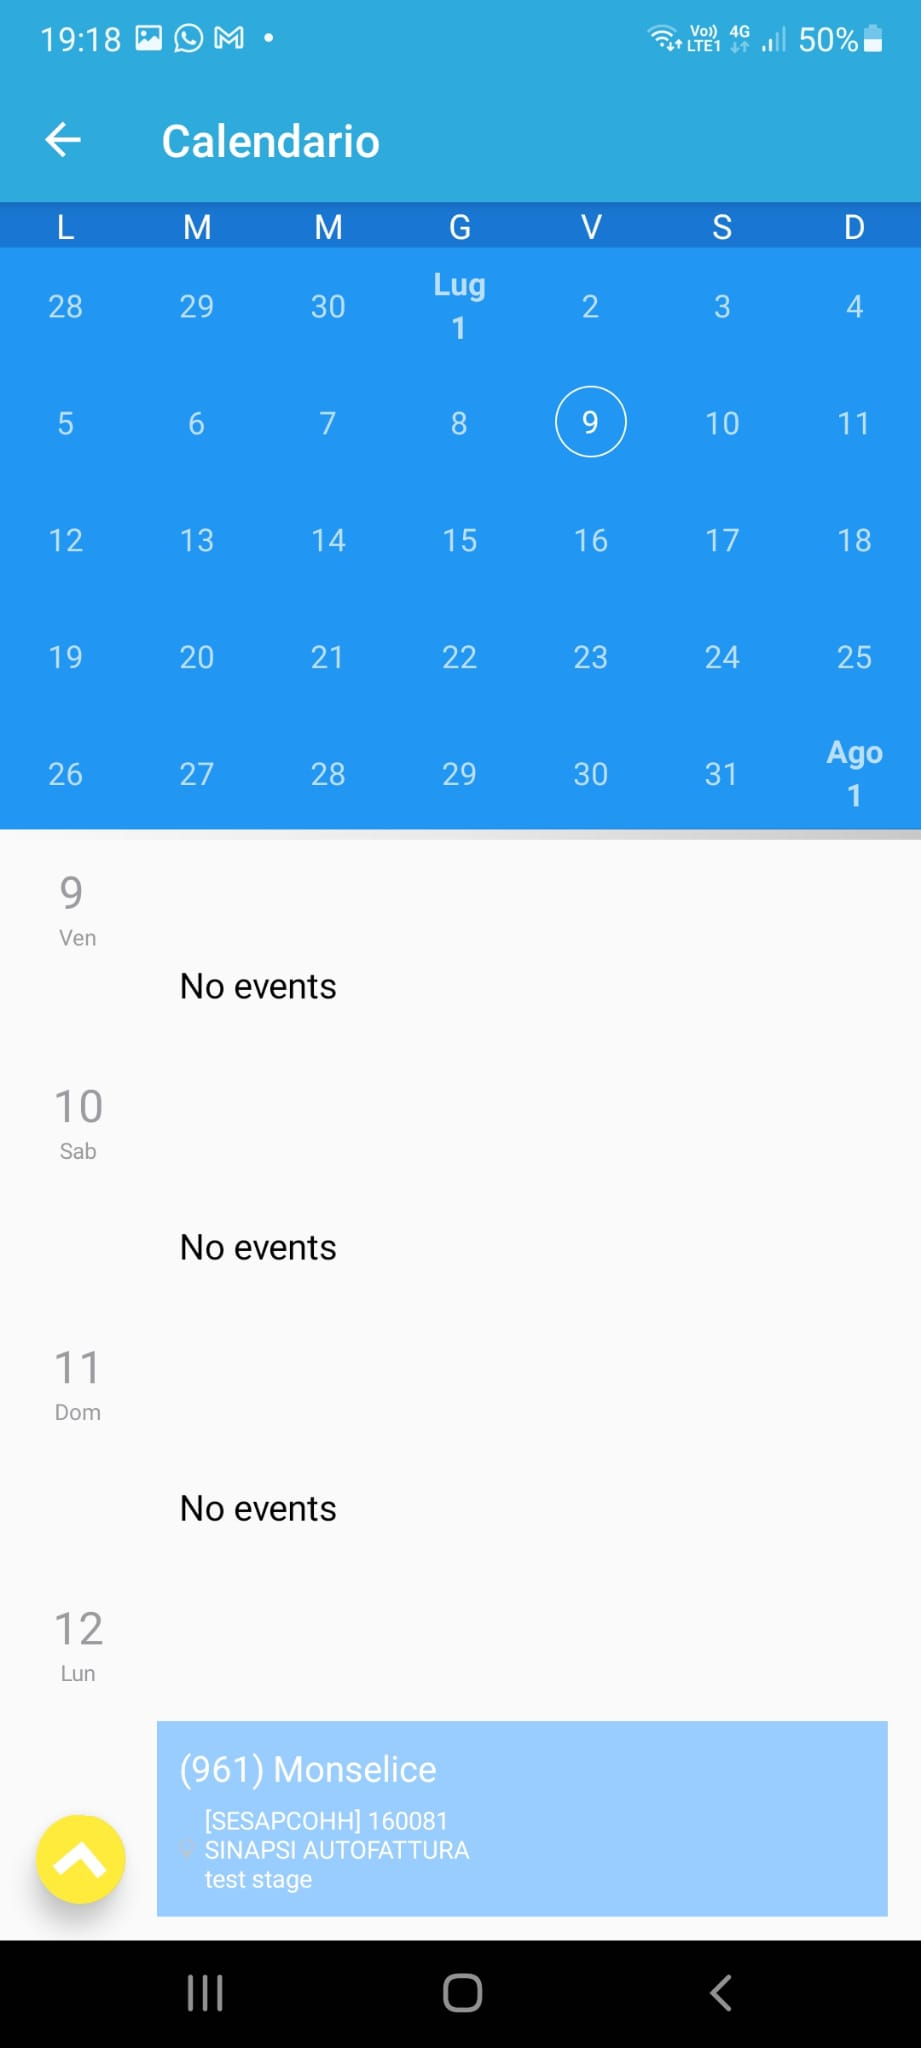
\includegraphics[scale = 0.11]{immagini/app Android/calendario-android.jpeg}
	\caption {App Android, schermata Calendario}
\end{figure}
\newpage
Infine, abbiamo i dettagli della chiamata di servizio selezionata.\\
\begin{figure}[!h] 
	\centering 
	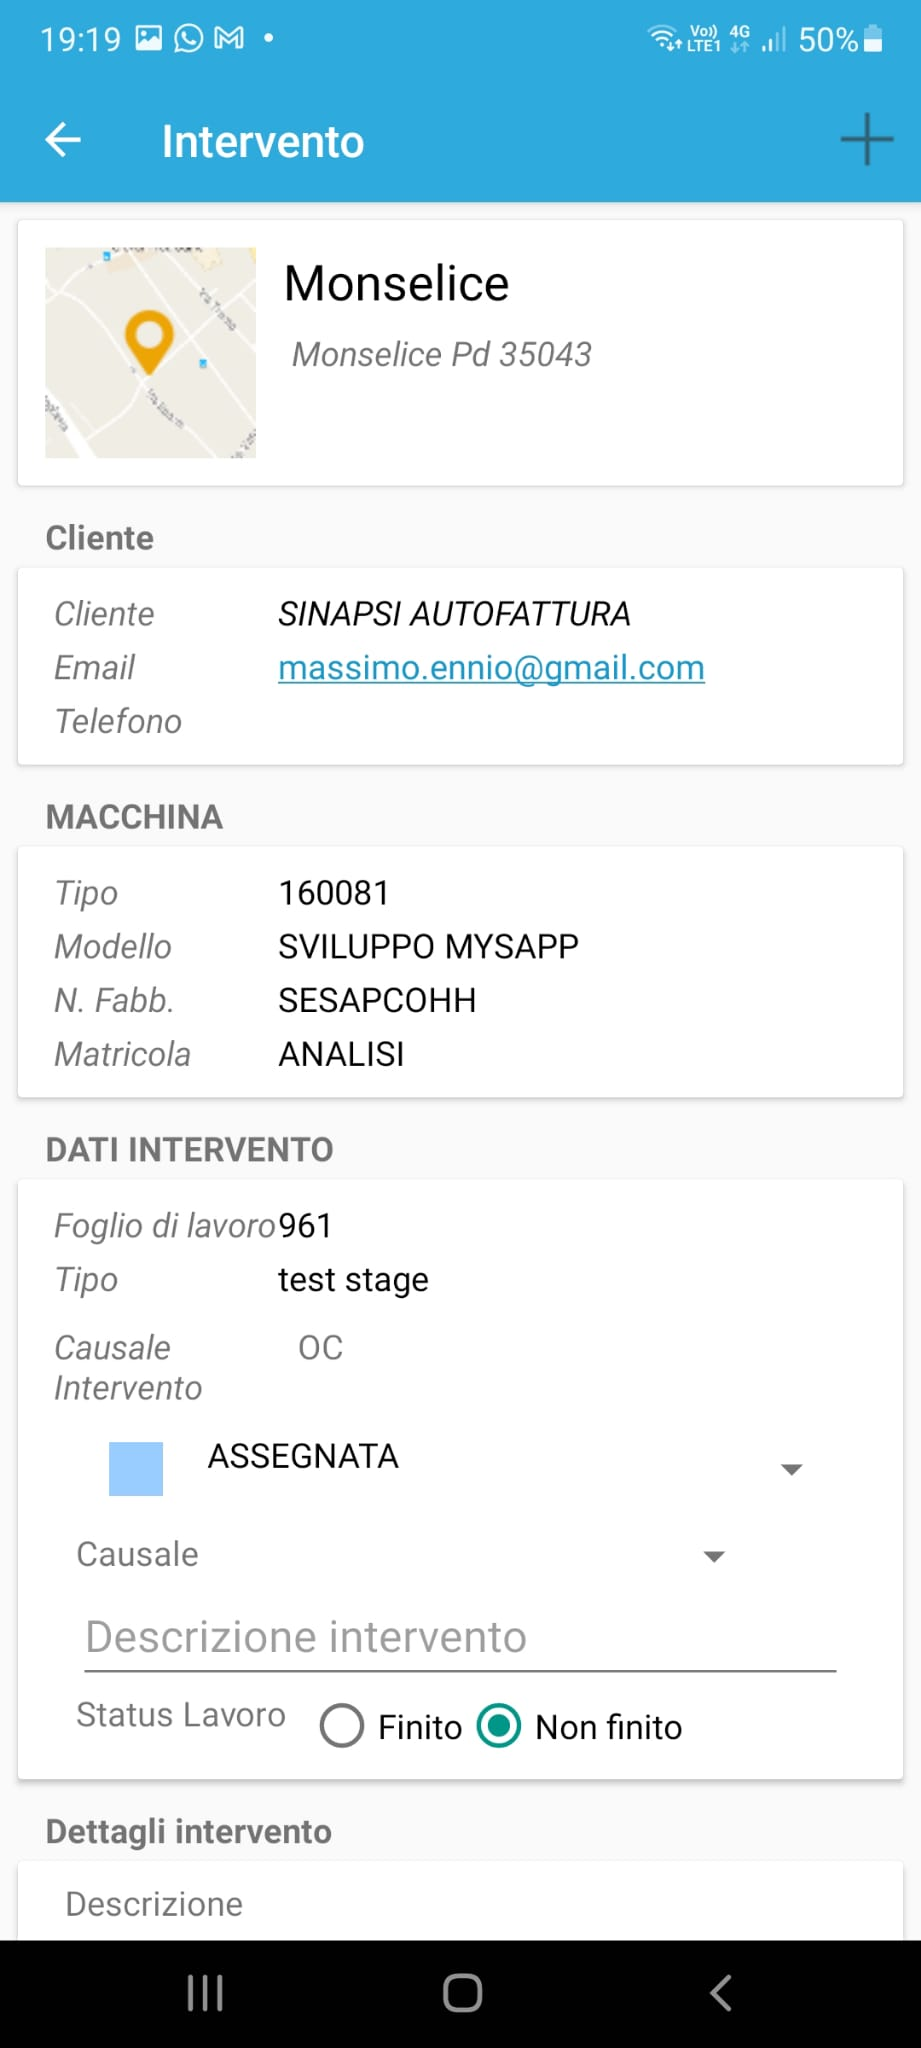
\includegraphics[scale = 0.2]{immagini/app Android/intervento-android.jpeg} 
	\caption {App Android, schermata Intervento}
\end{figure}
\\Qui possiamo vedere i vari dettagli della chiamata di servizio, ad esempio:
\begin{itemize}
	\item posizione del cliente;
	\item attrezzatura che necessita dell'intervento;
	\item dati e dettagli dell'intervento.
\end{itemize}
\newpage             % Processi
	% !TEX encoding = UTF-8
% !TEX TS-program = pdflatex
% !TEX root = ../tesi.tex

%**************************************************************
\chapter{Descrizione dello stage}
\label{cap:descrizione-stage}
%**************************************************************

\intro{In questo capitolo descriveremo gli obiettivi e il lavoro effettuato nello stage a grandi linee, per poi approfondire nel dettaglio nei prossimi capitoli}\\

%**************************************************************
\section{Introduzione al progetto}
\begin{figure}[!h] 
	\centering 
	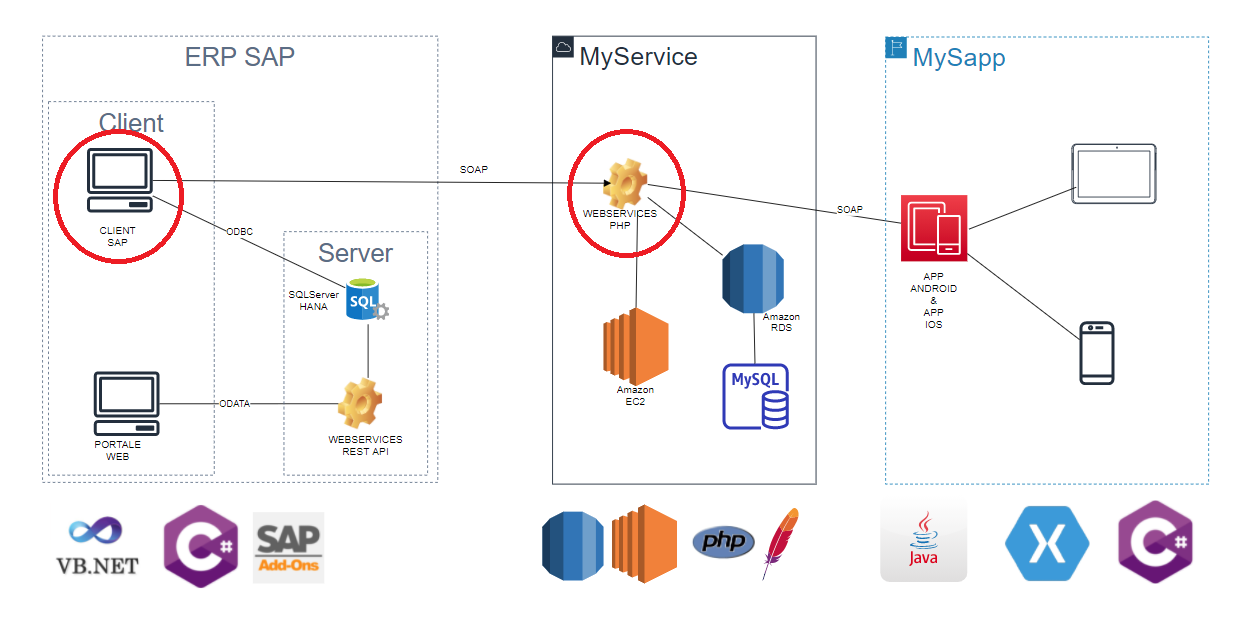
\includegraphics[scale = 0.5]{immagini/obiettivi-stage.png} 
	\caption{Schema infrastruttura preesistente, con evidenziati le componenti obiettivo del lavoro di stage}
	\label{fig:3-1}
\end{figure}
\newpage
\begin{flushleft}
	In figura \ref{fig:3-1} possiamo vedere lo schema dell'infrastruttura preesistente, già vista nel capitolo precedente.\\
	Evidenziate in rosso, con un cerchio, possiamo vedere le due componenti su cui è stato concentrato il lavoro durante questo stage:
\end{flushleft}

\begin{itemize}
	\item \textbf{Client SAP:} è stato creato un nuovo add-on, utilizzabile dal client SAP;
	\item \textbf{Webservices PHP:} sono state modificate ed ampliate alcune funzioni che compongono i webservices in PHP.
\end{itemize}
\subsection{Vincoli tecnologici}
L'azienda ha posto due vincoli tecnologici:
\begin{itemize}
	\item nello sviluppo dell'add-on, utilizzare VB.NET oppure C\#;
	\item negli ampliamenti dei webservices solamente il linguaggio PHP.
\end{itemize}
Il vincolo sugli add-on è tale, poichè quest'ultimi possono essere programmati soltanto in quei due linguaggi.

Il vincolo sugli ampliamenti dei webservices è dettato dal dover modificare delle funzioni in PHP, dunque bisogna utilizzare lo stesso linguaggio.
\section{Interazione}
Per lo svolgimento dell'attività di stage si è deciso in comune accordo con il tutor aziendale di svolgere lo stage completamente in azienda.\\
Questo è stato deciso per favorire il dialogo tra studente e tutor aziendale, ed eventualmente un confronto con gli altri dipendenti dell'azienda, esperti nel settore d'interesse.
\section{Requisiti e obiettivi}
Sin dal piano di lavoro sono stati decisi alcuni obiettivi, di cui 3 obbligatori e 1 desiderabile.
\\Obiettivi obbligatori:
\begin{itemize}
	\item Comprensione e apprendimento di strumenti di programmazione e infrastruttura esistente;
	\item Sviluppo protocolli di comunicazione tra i diversi moduli;
	\item Sviluppo applicazione add-on.
\end{itemize}
Obiettivo desiderabile:
\begin{itemize}
	\item Test e documentazione.
\end{itemize}
\subsection{Raggiungimento obiettivi}
Gli obiettivi e risultati raggiunti dall'applicazione sono stati considerati più che sufficienti dall'azienda.
In particolare sono stati raggiunti tutti gli obiettivi obbligatori concordati nel piano di lavoro.

Purtroppo non è stato possibile effettuare test automatici del codice, poichè il codice non è abbastanza corposo da renderli necessari.

%**************************************************************
\section{Pianificazione}
La durata dello stage è stimata attorno alle 320 ore circa.\\
Per ottenere una buona organizzazione dell'attività di stage, è stato stilato il piano di lavoro assieme al tutor aziendale Massimo Ennio e al relatore Massimiliano De Leoni.
\subsection{Piano di Lavoro}
La ripartizione delle ore è stata distribuita nelle 8 settimane in questo modo:
\begin{figure}[!h] 
	\centering 
	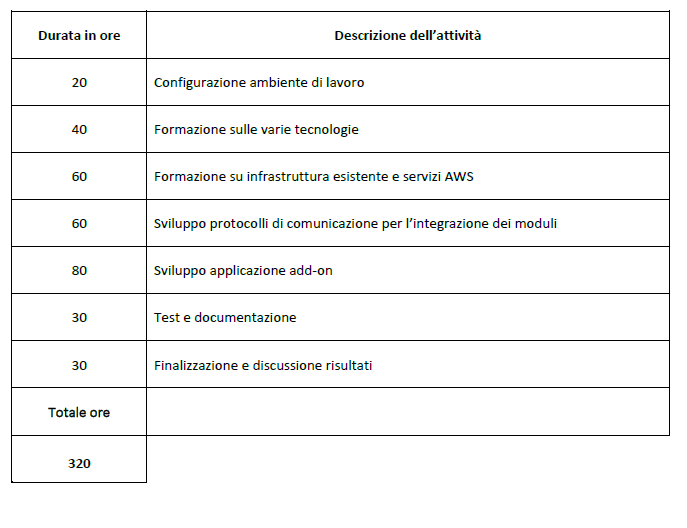
\includegraphics[scale = 0.8]{immagini/ripartizione-ore-piano.png} 
	\caption{Ripartizione ore, secondo il piano di lavoro, durante l'attività di stage}
\end{figure}

             % Kick-Off
	% !TEX encoding = UTF-8
% !TEX TS-program = pdflatex
% !TEX root = ../tesi.tex

%**************************************************************
\chapter{Sviluppo Add-On}
\label{cap:sviluppo-addon}
%**************************************************************

\intro{In questo capitolo approfondiremo lo sviluppo dell'add-on}


\section{Analisi dei requisiti}
\subsection{Introduzione}


	\item Fulcro dell'attività di stage è stata la produzione e sviluppo di un add-on, un'applicazione a maschera, applicabile al client SAP.
	
	Lo scopo di quest'add-on è la stampa di un form o tabella di un modulo di SAP, ad esempio il form Scheda Attrezzatura, oppure l'esportazione su file esterno.
	\item Quest'applicazione è stata codificata in Microsoft Visual Studio, con le librerie di SAP Business One, in linguaggio C\#.
	
	Per realizzarlo c'è stato un periodo di formazione personale sul linguaggio C\# e sulle librerie di SAP per lo sviluppo degli add-on.

\vspace{1em}


Continuiamo con la presentazione dei casi d'uso e il tracciamento dei requisiti.
\newpage

\subsection{Casi d'uso}

	Per lo studio dei casi di utilizzo del prodotto sono stati creati dei diagrammi.
	
	I diagrammi dei casi d'uso (in inglese \emph{Use Case Diagram}) sono diagrammi di tipo \gls{uml} dedicati alla descrizione delle funzioni o servizi offerti da un sistema, così come sono percepiti e utilizzati dagli attori che interagiscono col sistema stesso.



\begin{figure}[!h] 
	\centering 
	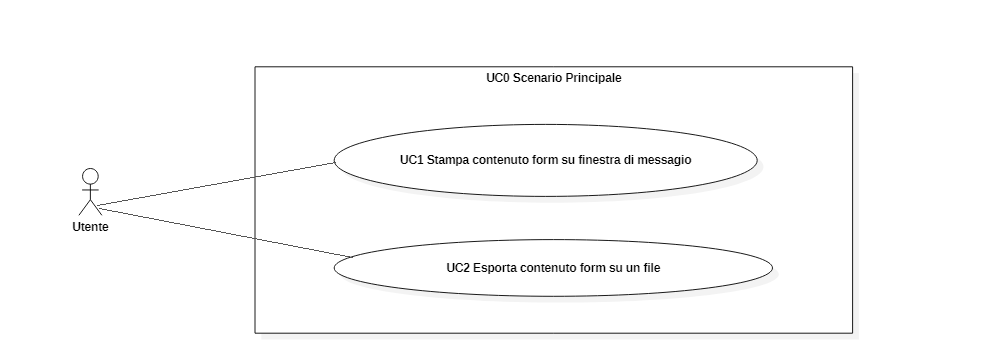
\includegraphics[scale = 0.4]{immagini/usecase/usecase-addon-uc0.png} 
	\caption{Use Case - UC0: Scenario principale}
\end{figure}
\begin{usecase}{0}{Scenario principale}
	\usecasepre{L'utente è entrato in un form del SAP}
	\usecasedesc{L'add-on mette a disposizione le funzionalità di stampa o salvataggio su file, dei contenuti del form}
	\usecasepost{Il sistema è pronto per permettere una nuova interazione}
	\label{uc:scenario-principale}
\end{usecase}
\begin{figure}[!h] 
	\centering 
	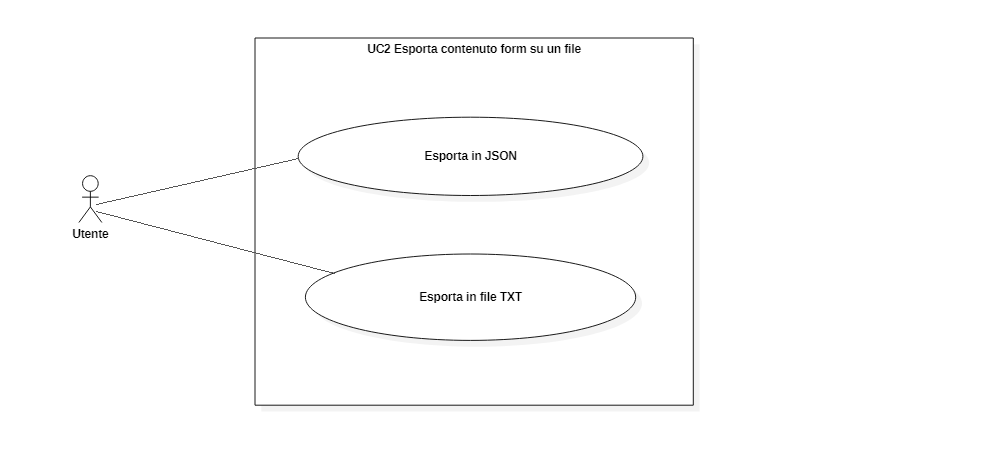
\includegraphics[scale = 0.4]{immagini/usecase/usecase-addon-uc2.png} 
	\caption{Use Case - UC2: Esporta contenuto form su un file}
\end{figure}
\begin{usecase}{2}{Esporta contenuto form su un file}
	\usecasepre{L'utente ha selezionato di salvare i contenuti del form su un file esterno}
	\usecasedesc{L'add-on metta a disposizione il salvataggio su file .txt o su file .json}
	\usecasepost{Il sistema è pronto per permettere una nuova interazione}
	\label{uc:esporta-file}
\end{usecase}

\newpage

\subsection{Tracciamento dei requisiti}
Da un'attenta analisi dei requisiti e degli use case effettuata sul progetto è stata stilata la tabella che traccia i requisiti in rapporto agli use case.

Sono stati individuati diversi tipi di requisiti e si è quindi fatto utilizzo di un codice identificativo per distinguerli.

Il codice dei requisiti è così strutturato R(F/Q/V)(O/D/F) dove:
\begin{enumerate}
	\item[R =] requisito
	\item[F =] funzionale
	\item[Q =] qualitativo
	\item[V =] di vincolo
	\item[O =] obbligatorio
	\item[D =] desiderabile
	\item[F =] facoltativo
\end{enumerate}
Nelle tabelle \ref{tab:requisiti-funzionali} e \ref{tab:requisiti-vincolo} sono riassunti i requisiti e il loro tracciamento con gli use case delineati in fase di analisi.


\begin{table}[!h]%
	\begin{tabularx}{\textwidth}{lXl}
		\hline\hline
		\textbf{Requisito} & \textbf{Descrizione} & \textbf{Use Case}\\
		\hline
		RFO-1     & L'add-on deve permettere di stampare il contenuto del form sotto forma di finestra di messaggio & UC1 \\
		RFO-2     & L'add-on deve permettere di esportare il contenuto del form in un file in formato JSON & UC2.1\\
		RFO-3     & L'add-on deve permettere di esportare il contenuto del form in un file in formato TXT & UC2.2\\
		\hline
	\end{tabularx}
	\caption{Tabella del tracciamento dei requisiti funzionali}
	\label{tab:requisiti-funzionali}
\end{table}%

\begin{table}[!h]%
	\begin{tabularx}{\textwidth}{lXl}
		\hline\hline
		\textbf{Requisito} & \textbf{Descrizione} & \textbf{Use Case}\\
		\hline
		RVO-1    & La versione di SAP Business One da utilizzare è la versione 10.0 & - \\
		\hline
	\end{tabularx}
	\caption{Tabella del tracciamento dei requisiti di vincolo}
	\label{tab:requisiti-vincolo}
\end{table}%

\newpage

\section{Realizzazione}

	Lo sviluppo dell'add-on è stato effettuato, come detto in precedenza, con linguaggio C\# e attraverso l'\gls{ide} Microsoft Visual Studio.
	
	Inoltre è stata usata una delle varie librerie fornite da SAP Business One SDK, ovvero:
	\begin{itemize}
		\item \textbf{SAPbouiCOM:} ovvero SAP Business One UI COM, una libreria COM di SAP Business One, per la gestione dell'interfaccia grafica(\emph{User Interface}).
	\end{itemize}
	Nella sezione precedente, non sono stati forniti diagrammi di classe poichè il codice dell'add-on, consiste in una classe che gestisce gli eventi generali ed una classe di supporto che gestisce gli eventi del form aperto.
	
	Dunque, essendo solo due classi, è stato ritenuto poco utile fornire diagrammi.
	
	\vspace{1em}
	Nel proseguo, viene illustrata una realizzazione tramite uno scenario di utilizzo.


	Per prima cosa accediamo al SAP con le credenziali corrette ed entriamo su un form, di un modulo.
	
	In questo caso entriamo nel form Scheda Attrezzatura, mostrato in figura \ref{fig:4-4}.
	

\begin{figure}[!h] 
	\centering 
	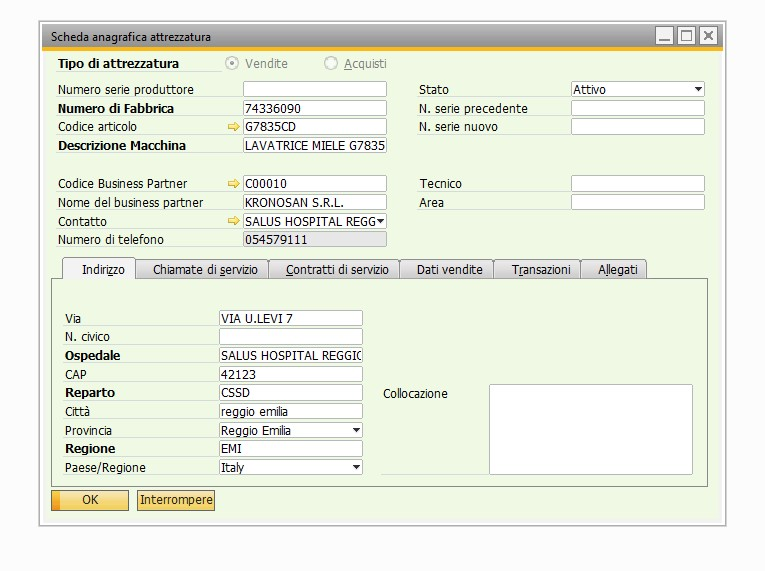
\includegraphics[scale = 0.6]{immagini/add-on/addon-scheda-nobutton.jpg} 
	\caption{Add-On, screenshot prima dell'attivazione dell'add-on}
	\label{fig:4-4}
\end{figure}
Come possiamo notare in figura \ref{fig:4-4} abbiamo due pulsanti:
\begin{itemize}
	\item Ok;
	\item Interrompere.
\end{itemize}

\newpage


	Ora attiviamo l'add-on:

\begin{itemize}
	\item installare l'add-on nel client SAP locale;
	\item compilare e farlo eseguire su Microsoft Visual Studio, senza averlo installato nel client SAP;
	\item nel caso sia installato nel client SAP, si può impostare l'attivazione manuale o automatica;
	\item nel caso di attivazione manuale, bisogna andare sulle opzioni degli add-on installati ed attivarlo.
\end{itemize} 

	
	Una volta attivato l'add-on, riapriamo il modulo Scheda Attrezzatura e vedremo comparire un pulsante nuovo.
	

\begin{figure}[!h] 
	\centering 
	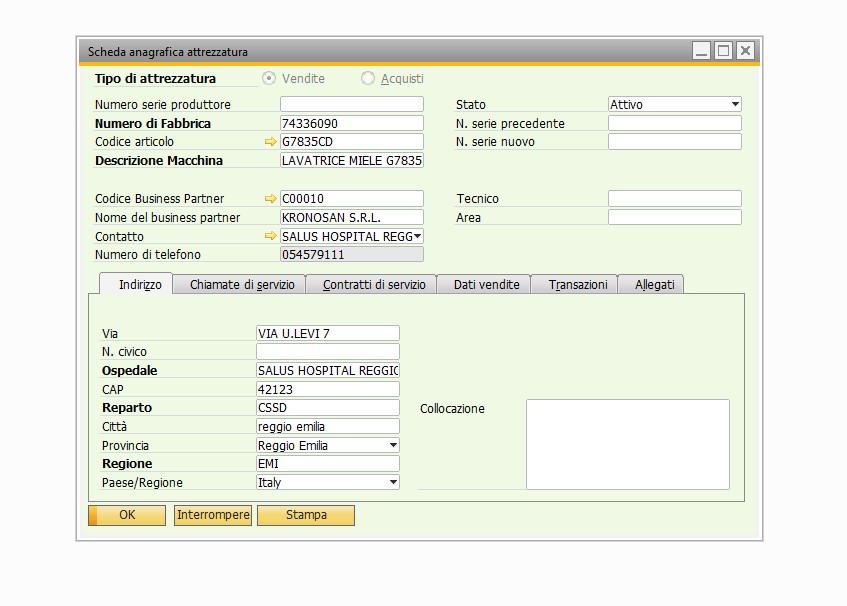
\includegraphics[scale = 0.6]{immagini/add-on/addon-scheda-yesbutton.jpg} 
	\caption{Add-On, screenshot dopo l'attivazione dell'add-on}
	\label{fig:4-5}
\end{figure}

	
	In figura \ref{fig:4-5} è già stata selezionata un'attrezzatura, in questo caso l'ultima attrezzatura aggiunta nel database.
	


\newpage

\vspace{1em}

Cliccando il pulsante Stampa si aprirà una nuova finestra.

\begin{figure}[!h] 
	\centering 
	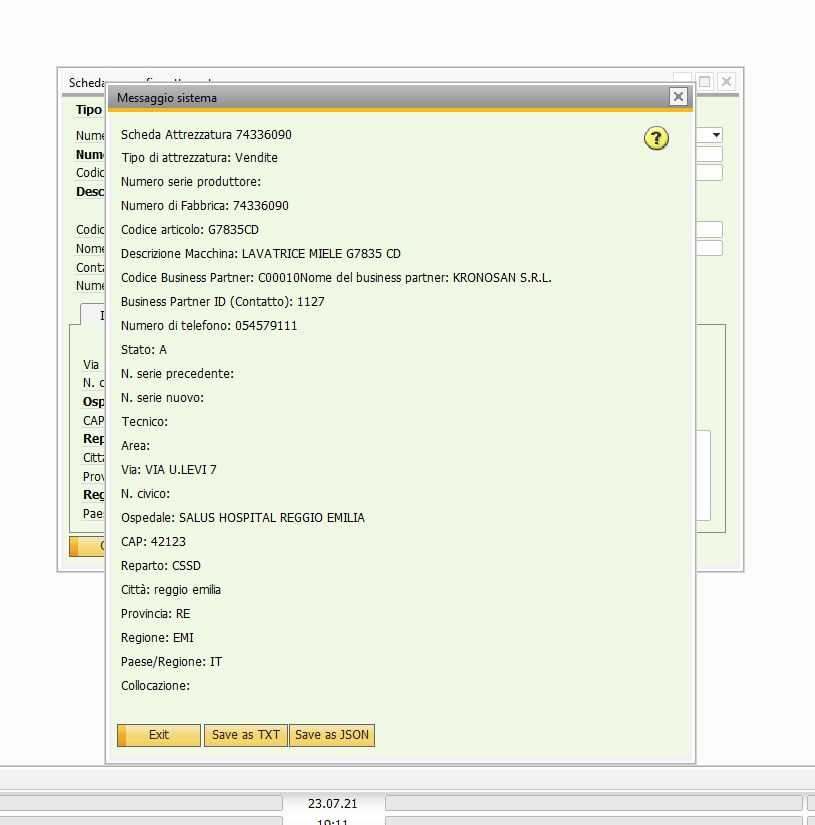
\includegraphics[scale = 0.6]{immagini/add-on/addon-stampa.jpg} 
	\caption{Add-On, stampa dei contenuti del form su finestra di messaggio}
	\label{fig:4-6}
\end{figure}

	
	Dopo aver cliccato il pulsante Stampa, si entra nella finestra mostrata in figura \ref{fig:4-6}, dove abbiamo stampato su finestra di messaggio i contenuti del form; inoltre abbiamo altri 3 pulsanti:

\begin{itemize}
	\item \textbf{Exit:} premendo questo pulsante, come dice il nome, usciremo da questa finestra;
	\item \textbf{Save as TXT:} premendo questo pulsante il contenuto di questa finestra verrà esportato su un file .txt, senza alcuna formattazione aggiuntiva;
	\item \textbf{Save as JSON:} premendo questo pulsante il contenuto di questa finestra verrà esportato su un file .json, con la formattazione json.
\end{itemize}


	I file vengono salvati nella cartella dov'è installato l'add-on, in particolare vengono chiamati rispettivamente \textbf{file.txt} per il file TXT e \textbf{filejson.json} per il file JSON.
	
	Se questi file esistono già nella cartella, e viene premuto nuovamente il pulsante di salvataggio, i file verranno sovrascritti dall'ultimo file.
	


\newpage


	
	Ora nei prossimi due screenshot, vedremo il contenuto dei due file, rispettivamente txt e json, esportati dall'add-on.
	

\begin{figure}[!h] 
	\centering 
	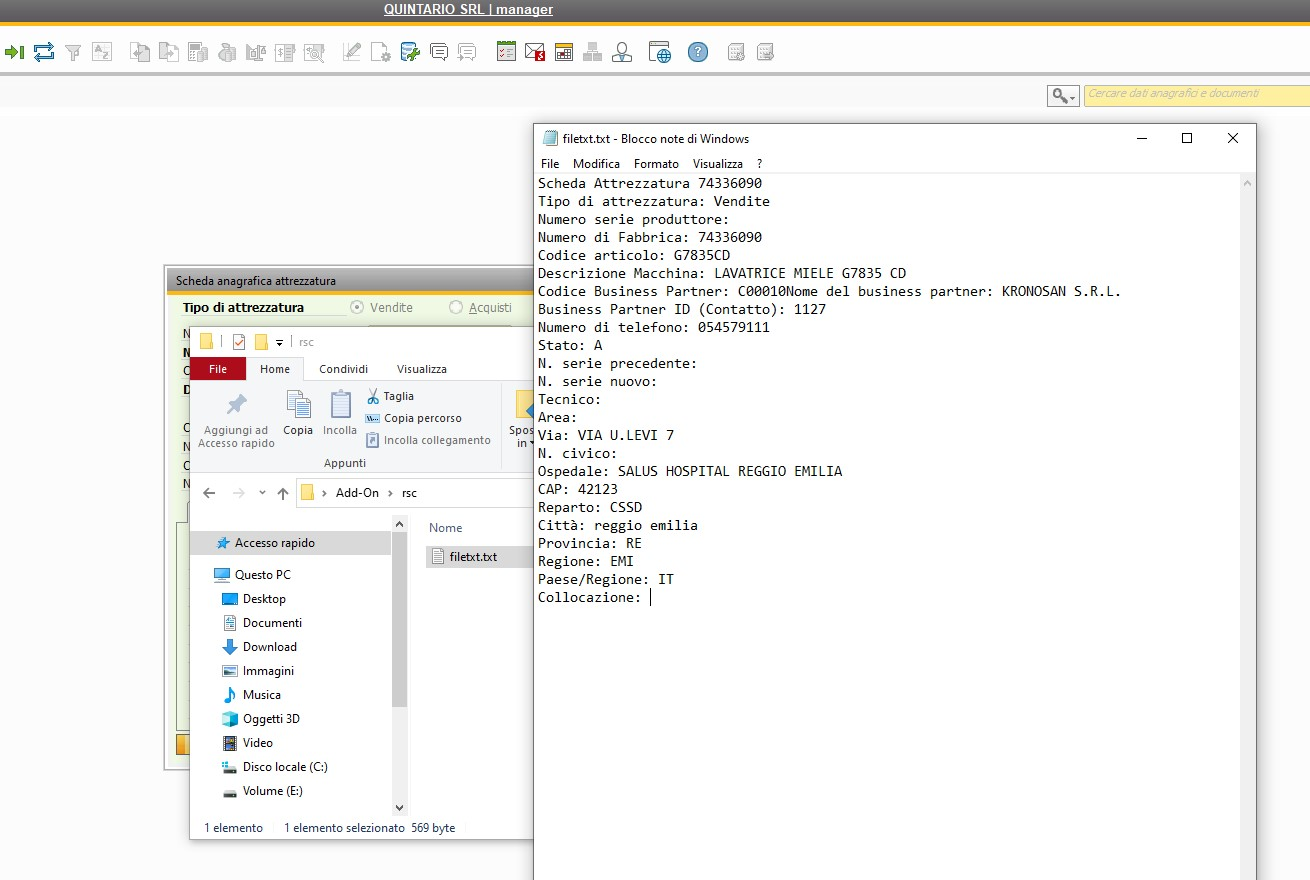
\includegraphics[scale = 0.38]{immagini/add-on/addon-esporta-txt.jpg} 
	\caption{Add-On, file txt esportato dall'add-on}
\end{figure}

\begin{figure}[!h] 
	\centering 
	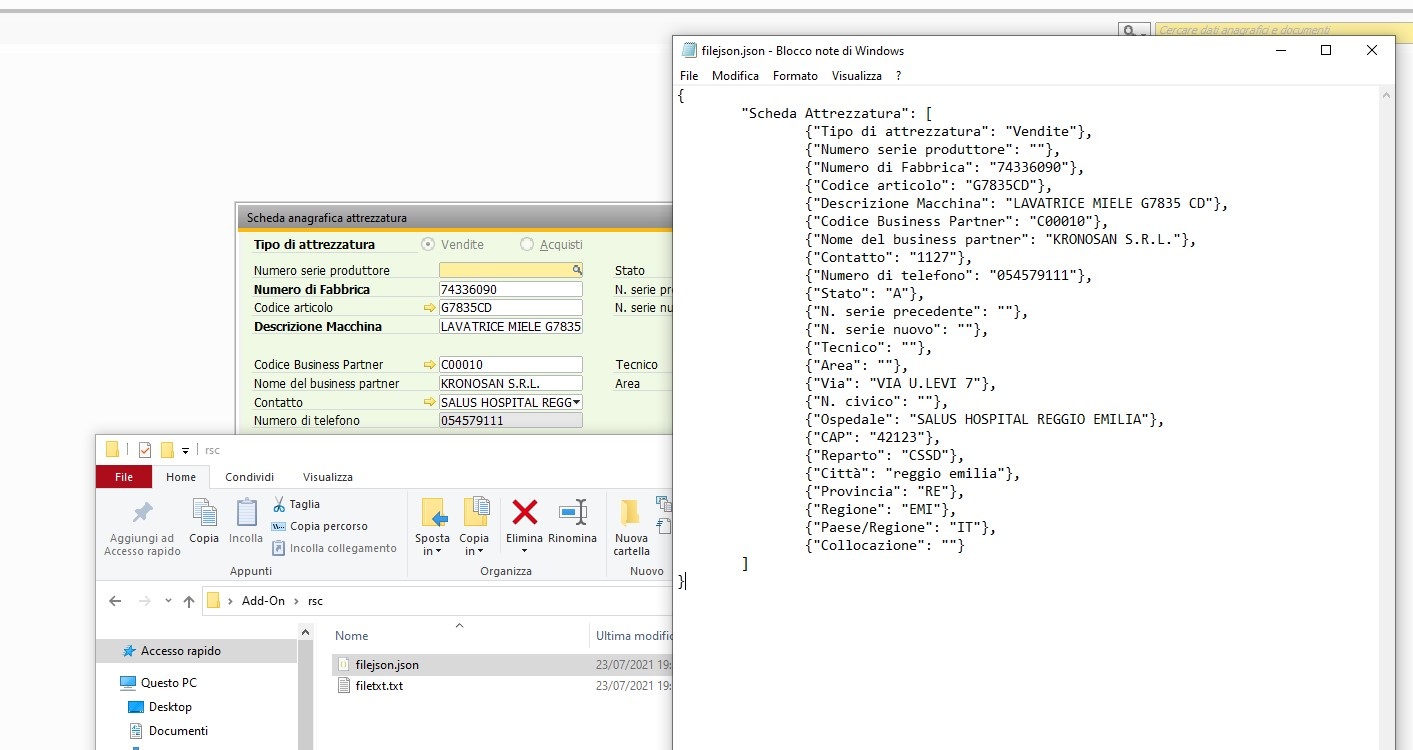
\includegraphics[scale = 0.38]{immagini/add-on/addon-esporta-json.jpg} 
	\caption{Add-On, file json esportato dall'add-on}
\end{figure}

\newpage

\section{Accettazione}


Riguardo la Verifica e Validazione, ovvero l'Accettazione, non abbiamo alcun test d'unità e test automatico.
Dunque per verificare l'add-on abbiamo una sequenza di operazioni da eseguire per verificarne il corretto funzionamento.
\vspace{1em}


La procedura per verificare il corretto funzionamento dell'applicazione è la seguente:



\begin{enumerate}
	\item Accedere al SAP Business One con le proprie credenziali;
	\item Attivare l'add-on dalle opzioni del client;
	\item Aprire il form Scheda Attrezzatura nel modulo dei Servizi;
	\item Selezionare un'istanza di attrezzatura esistente, usualmente attraverso il numero di fabbrica, essendo chiave univoca di questa tabella;
	\item Cliccare il pulsante Stampa;
	\item Verificare che le informazioni stampate nella nuova finestra di messaggio apertasi corrispondano alle informazioni del form;
	\item Cliccare Save as JSON;
	\item Cliccare Save as TXT;
	\item Entrare nella cartella dell'add-on dove sono salvati i file;
	\item Verificare che il contenuto dei file corrisponda alle informazioni del form.
\end{enumerate}

Se non ci sono stati problemi in questi step, in particolare se le informazioni stampate nella finestra di messaggio e le informazioni salvate nei due file corrispondono alle informazioni presenti nel form Scheda anagrafica attrezzatura, l'add-on può considerarsi verificato e validato.

\subsection{Requisiti soddisfatti}
Logicamente i requisiti funzionali sono stati tutti soddisfatti, eccone qui una piccola tabella.

\begin{table}[!h]%
	\begin{tabularx}{\textwidth}{lXl}
		\hline\hline
		\textbf{Requisito} & \textbf{Descrizione} & \textbf{Use Case}\\
		\hline
		RFO-1     & Step 6 & Soddisfatto \\
		RFO-2     & Step 10 & Soddisfatto\\
		RFO-3     & Step 10 & Soddisfatto\\
		\hline
	\end{tabularx}
	\caption{Tabella del soddisfacimento dei requisiti funzionali}
	\label{tab:requisiti-funzionali-soddisfatti}
\end{table}%             % Concept Preview
	% !TEX encoding = UTF-8
% !TEX TS-program = pdflatex
% !TEX root = ../tesi.tex

%**************************************************************
\chapter{Progettazione e codifica}
\label{cap:progettazione-codifica}
%**************************************************************

\intro{Breve introduzione al capitolo}\\

%**************************************************************
\section{Tecnologie e strumenti}
\label{sec:tecnologie-strumenti}

Di seguito viene data una panoramica delle tecnologie e strumenti utilizzati.

\subsection*{Tecnologia 1}
Descrizione Tecnologia 1.

\subsection*{Tecnologia 2}
Descrizione Tecnologia 2

%**************************************************************
\section{Ciclo di vita del software}
\label{sec:ciclo-vita-software}

%**************************************************************
\section{Progettazione}
\label{sec:progettazione}

\subsubsection{Namespace 1} %**************************
Descrizione namespace 1.

\begin{namespacedesc}
    \classdesc{Classe 1}{Descrizione classe 1}
    \classdesc{Classe 2}{Descrizione classe 2}
\end{namespacedesc}


%**************************************************************
\section{Design Pattern utilizzati}

%**************************************************************
\section{Codifica}
             % Product Prototype
	% !TEX encoding = UTF-8
% !TEX TS-program = pdflatex
% !TEX root = ../tesi.tex

%**************************************************************
\chapter{Conclusioni}
\label{cap:conclusioni}
%**************************************************************
\intro{In questo capitolo finale viene verificato il raggiungimento degli obiettivi prestabiliti e vengono fatte delle considerazioni sullo stato attuale del programma}
%**************************************************************
\section{Raggiungimento degli obiettivi}


Gli obiettivi e risultati raggiunti dall'applicazione sono stati considerati più che sufficienti dall'azienda.

In particolare sono stati raggiunti tutti gli obiettivi obbligatori concordati nel piano di lavoro.

Purtroppo non è stato possibile effettuare test automatici del codice, poichè il codice non è abbastanza corposo da renderli necessari.

I file prodotti e la stampa su finestra di messaggio sono risultati conforme alle aspettative e ne è stata verificata la correttezza.



%**************************************************************
\section{Conoscenze acquisite}
Le conoscenze acquisite sono state molteplici, a partire da nuovi linguaggi di programmazione al mondo dei gestionali e a tutte le applicazioni di supporto che permettono di far funzionare tutto il sistema con efficienza.

In particolare, le conoscenze acquisite principalmente sono:
\begin{itemize}
    \item \textbf{Conoscenze sul gestionale SAP Business One: }Uno studio approfondito della documentazione SAP presente online, e uno studio parallelo su ambienti di test SAP, per testare le conoscenze via via acquisite dalla documentazione;
    \item \textbf{Conoscenze acquisite su applicazioni di supporto: } Molte nuove conoscenze su applicazioni come SQL Server Management Studio, Postman, SoapUI, HeidiSQL e Remote Desktop per gestire le varie parti dell'infrastruttura presistente;
    \item \textbf{Conoscenze acquisite su C\# e librerie di SAP relative: } Uno studio della \textit{Software Development Kit}, in breve SDK, fornita da SAP Business One, ovvero le librerie SAP per programmare gli add-ons, e l'applicazione di queste librerie su codice in C\#;
    \item \textbf{Conoscenze acquisite su PHP: } L'aver ampliato notevolmente le conoscenze nel linguaggio PHP, dato il lavoro di ampliamento su un codice già complesso e strutturato, con necessario studio e comprensione profonda di questo codice preesistente.
\end{itemize}

%**************************************************************
\section{Esperienza di stage}

Nel complesso l'esperienza di studio dell'infrastruttura preesistente e sviluppo dell'add-on si è rivelata molto formativa.

Ma senza ombra di dubbio l'ampliamento delle funzioni PHP per i webservices è stata altamente formativa.

\newspace

Sono soddisfatto di questo progetto, poichè sono riuscito a comprendere un po' il mondo dei gestionali e soprattutto quanta conoscenza ci sia ancora da apprendere su questo campo.

Sono soddisfatto della parte tecnologica dell'attività di stage in quanto mi ha permesso di imparare C\# e approfondire il linguaggio PHP, e di applicare le mie conoscenze di SQL.

\newspace

Ho potuto godere di un'ampia autonomia nella gestione ed organizzazione del mio lavoro, nel rispetto di vincoli e funzionalità stabilite ad inizio progetto.

Grazie a questa esperienza di stage ho potuto integrarmi e confrontarmi con una realtà molto diversa da quella che ero abituato a vedere e relazionarmi con persone che vedono le cose sotto un altro punto di vista.

Particolarmente importante è stata la collaborazione con i capi progetto e con i vari dipendenti dell'azienda. \'E stato essenziale il supporto che mi hanno fornito nell'ambientamento e nella comprensione dei nuovi argomenti, differenti da quelli studiati nel mio percorso scolastico.
             % Conclusioni                              
	
	%**************************************************************
	% Materiale finale
	%**************************************************************
	\backmatter
	\printglossaries
	% !TEX encoding = UTF-8
% !TEX TS-program = pdflatex
% !TEX root = ../tesi.tex

%**************************************************************
% Bibliografia
%**************************************************************

\cleardoublepage
\chapter{Bibliografia}

\nocite{*}
% Stampa i riferimenti bibliografici
\printbibliography[heading=subbibliography,title={Riferimenti bibliografici},type=book]

% Stampa i siti web consultati
\printbibliography[heading=subbibliography,title={Siti web consultati},type=online]


\end{document}
